\documentclass[%
    school=etsisi,%
    type=pfg,%
    degree=61TI,%
    authorsex=m,%
    directorsex=m,%
]{upm-report}

\usepackage{wrapfig}

\addbibresource{references.bib}

\author{Marcos Martínez Francisco}
\title{Consensus Mechanisms in the Cosmos SDK and Their Applications in Private Blockchains}
\director{Sergio Arévalo, Ernesto Jiménez}

\abstract{spanish}{
Esta tesis presenta un estudio exhaustivo del Cosmos SDK y su aplicación en el desarrollo de blockchains privadas. Explora varios mecanismos de consenso dentro del Cosmos SDK, como BFT, PBFT y DPoS, evaluando sus propiedades de seguridad, escalabilidad y descentralización. Además, profundiza en el diseño e implementación de blockchains privadas, enfatizando un caso de estudio sobre crowdfunding. 

Este trabajo busca iluminar el potencial del Cosmos SDK para crear soluciones de blockchain privadas eficientes, seguras y personalizables, destacando sus ventajas sobre los marcos de blockchain tradicionales. La tesis también sugiere direcciones para futuras investigaciones en el mejoramiento de las capacidades del Cosmos SDK en aplicaciones de blockchain privadas.}
\keywords{spanish}{Cosmos SDK; Golang; Blockchain; Decentralization; Private Blockchains}

\abstract{english}{
This thesis presents an extensive study of the Cosmos SDK and its application in private blockchain development. It explores the various consensus mechanisms within the Cosmos SDK, such as BFT, PBFT, and DPoS, assessing their security, scalability, and decentralization properties. 

The work further delves into the design and implementation of private blockchains, particularly emphasizing a case study on crowdfunding. This research aims to illuminate the potential of the Cosmos SDK in creating efficient, secure, and customizable private blockchain solutions, highlighting its advantages over traditional blockchain frameworks. The thesis also suggests directions for future research in enhancing the capabilities of the Cosmos SDK in private blockchain applications.}
\keywords{english}{Cosmos SDK; Golang; Blockchain; Decentralization;Private Blockchains}

\acknowledgements{
   To my mother.
 }

\begin{document}

\newglossaryentry{RESTful}{
        name=RESTful,
        description={Architectural style for an application program interface that uses HTTP requests to access and use data}
}

\newglossaryentry{Blockchain}{
        name=Blockchain,
        description={Distributed database or ledger that is shared among the nodes of a computer network}
}

\newacronym{nft}{NFT}{Non Fungible Token}
\newacronym{defi}{DeFi}{Decentralized Finance}
\newacronym{poa}{PoA}{Proof of Authority}
\newacronym{pos}{PoS}{Proof of Stake}  
\newacronym{bft}{BFT}{Byzantine Fault Tolerance}
\newacronym{abci}{ABCI}{Application Blockchain Interface}
\newacronym{pbft}{PBFT}{Practical Byzantine Fault Tolerance}
\newacronym{pow}{PoW}{Proof of Work}
\newacronym{dpos}{DPoS}{Delegated Proof of Stage}
\newacronym{dag}{DAG}{Directed Acyclic Graph}
\newacronym{grpc}{gRPC}{Google Remote Procedure Call}
\newacronym{cli}{CLI}{Command Line Interface}
\newacronym{p2p}{P2P}{Peer to Peer}
\newacronym{dlt}{DLT}{Distributed Ledger Technology}
\newacronym{rpc}{RPC}{Remote Procedure Call}
\newacronym{cicd}{CI/CD}{Continuous Integration/Continuous Deployment}
\newacronym{os}{OS}{Operating System}
\newacronym{ibc}{IBC}{ Inter-Blockchain Communication}
\newacronym{dapps}{dApps}{Decentralized Applications}

\frontmatter

\begin{KeepFromToc}
  \tableofcontents
\end{KeepFromToc}

\begin{KeepFromToc}
  \listoffigures
\end{KeepFromToc}

\begin{KeepFromToc}
  \lstlistoflistings
\end{KeepFromToc}


\mainmatter

\chapter{Introduction}
\label{ch:introduccion}

The Cosmos SDK represents a paradigm shift in the world of blockchain technology. As an open-source framework for blockchain development, it emphasizes customization and efficiency, making the creation of tailored blockchain applications more accessible. Central to this framework is the Tendermint consensus mechanism, a rapid and secure proof-of-stake methodology, which serves as the backbone of the Cosmos SDK. This technology allows developers to focus more on developing the application layer, a topic we will delve into in Chapter \ref{OCS:overview}.

The adoption of private blockchains has seen a significant rise recently, especially among businesses and organizations. These entities are increasingly recognizing the benefits of blockchain technology, such as enhanced efficiency, privacy, and control, which are not always feasible with public blockchains. The Cosmos SDK, with its modular and adaptable design, emerges as an ideal solution for crafting private blockchain applications, addressing specific needs and challenges unique to these entities.

In this thesis, we will explore the technical intricacies of the Cosmos SDK and the Tendermint consensus mechanism. We will evaluate their strengths and limitations, and discuss their practical applications, particularly in the context of private blockchains. To illustrate the practicality and real-world application of this framework, a case study of a private blockchain developed using the Cosmos SDK will be presented.

\section{Background and Motivation}

Blockchain technology, with its potential to disrupt and transform various industries, has garnered considerable attention in recent years. My engagement in this field, through projects involving \gls{nft}, smart contracts, and \gls{defi} protocols, has led me to appreciate the broader scope and potential of blockchain technology beyond these initial applications.

This technology's ability to empower individuals, streamline transactions, and promote financial inclusion, especially in underbanked regions, drives its transformative potential. This thesis is motivated by a desire to explore and elucidate the capabilities of the Cosmos SDK and Tendermint in fostering private blockchains. It aims to contribute to the expanding research landscape on blockchain technology, particularly in its application beyond public blockchain frameworks.

\section{Document structure}

This thesis is organized as follows:

\begin{itemize}
    \item Section \ref{OCS:overview} provides a comprehensive overview of the Cosmos SDK, detailing its architecture and how it facilitates blockchain development.
    \item Section \ref{ch:compare} compares various consensus algorithms, assessing their applicability across different use cases.
    \item Section \ref{ch:private} outlines the process of designing a private blockchain, complemented by a real-world application case.
    \item Section \ref{ch:conclusion} concludes the thesis, summarizing the key concepts and suggesting avenues for future research.
\end{itemize}

\chapter{Blockchain Technology: Foundations and Applications}
\label{chap:blockchain_technology}

Blockchain technology, a decentralized digital ledger system, has emerged as a foundational technology that underpins cryptocurrencies like Bitcoin and extends far beyond to various sectors including finance, supply chain, and beyond. This chapter introduces blockchain technology, explores its key components, and lays the foundation for understanding its application within the Cosmos SDK.

\section{Introduction to Blockchain}
Blockchain technology offers a robust, secure, and transparent way to record transactions across a distributed network of computers. It eliminates the need for central authorities or intermediaries, enabling direct peer-to-peer interactions. The essence of blockchain technology lies in its ability to ensure the integrity and security of data without a central point of control, making it revolutionary for digital transactions and record-keeping \cite{nakamoto2008bitcoin, tapscott2016blockchain}.

\section{Key Components of Blockchain Technology}
A blockchain comprises several key components: blocks, transactions, and the consensus mechanism. Each block contains a collection of transactions that are verified and secured through cryptographic techniques. The blockchain utilizes a consensus mechanism, such as \gls{pow} or \gls{pos}, to agree on the validity of transactions and blocks, as shown in Lst~\ref{lst:state-transition}, ensuring all participants maintain a consistent state of the ledger~\cite{antonopoulos2014mastering, buterin2014next}.

\section{Decentralization and Security}
At the heart of blockchain technology is the principle of decentralization, which distributes control and decision-making across the network, reducing reliance on a single entity and enhancing security. This decentralization is bolstered by cryptographic algorithms, including hash functions and digital signatures, safeguarding against unauthorized tampering and ensuring the authenticity of transactions \cite{narayanan2016bitcoin}.

\section{Smart Contracts and DApps}

Blockchain technology introduces the concept of smart contracts, self-executing contracts with the terms of the agreement directly written into code. These smart contracts enable the development of \gls{dapps} that run on blockchain platforms, offering a wide range of applications beyond simple transactions \cite{szabo1997formalizing, wood2014ethereum}. The Ethereum platform, in particular, has popularized the use of smart contracts through the \gls{evm}.

\subsection{Ethereum Virtual Machine}

The \gls{evm} is a powerful, sandboxed virtual stack embedded within each Ethereum node, offering a controlled environment in which smart contracts run. The \gls{evm} executes bytecode, which is compiled from the high-level languages developers write smart contracts in, such as Solidity. This approach to smart contract deployment ensures that contracts are executed exactly as programmed, without any possibility of downtime, censorship, fraud, or third-party interference.

\subsection{Immutability and Development Challenges}

One of the core features of blockchain technology is the immutability of smart contracts. Once a contract is deployed on the blockchain, its code cannot be altered, making bug fixes or updates a significant challenge. This immutability ensures security and trust in the deployed contracts but introduces challenges in the development lifecycle, including:

\begin{itemize}
    \item \textbf{Upgradability:} Developers must design contracts with future updates in mind, often through indirect mechanisms like proxy contracts or by embedding upgrade logic within the contract itself.
    \item \textbf{Security:} Given the immutable nature of contracts, security vulnerabilities can be catastrophic. This necessitates thorough testing and auditing of contract code before deployment.
    \item \textbf{Versioning:} Managing different versions of contracts and ensuring compatibility between them becomes increasingly complex, especially as the ecosystem grows.
\end{itemize}

\subsection{Comparison with Cosmos SDK}

The Cosmos SDK offers a different approach to building blockchain applications, focusing on modularity and interoperability. Unlike the \glspl{evm} focus on a singular, immutable smart contract platform, the Cosmos SDK allows developers to build entire blockchains tailored to specific applications. This flexibility offers several advantages:

\begin{itemize}
    \item \textbf{Upgradability:} Cosmos SDK blockchains can be upgraded more easily, allowing developers to fix bugs or introduce new features without the constraints of contract immutability.
    \item \textbf{Customizability:} Developers have greater freedom to design the underlying blockchain logic and consensus mechanisms to best fit their application's needs.
    \item \textbf{Interoperability:} Through the \gls{ibc}, Cosmos SDK blockchains can communicate and transfer assets between one another, enabling a network of interoperable blockchains.
\end{itemize}

While both approaches offer unique advantages, the Cosmos SDK's flexibility and focus on interoperability provide a compelling framework for developing blockchain applications, especially for complex and evolving use cases. More details on the Cosmos SDK will be discussed in subsequent sections.


\section{Challenges and Future Directions}

While blockchain technology offers significant advantages, it also faces challenges, including scalability, energy consumption, and regulatory issues. Addressing these challenges is crucial for the widespread adoption of blockchain technology. The ongoing research and development in blockchain technology, including the exploration of more efficient consensus mechanisms and scaling solutions, indicate a promising future for this technology in various domains \cite{croman2016scaling, swan2015blockchain}.

This chapter has provided a foundational understanding of blockchain technology, emphasizing its decentralization, security features, and potential for innovation through smart contracts and \gls{dapps}. As we delve deeper into the Cosmos SDK in the following chapters, this foundational knowledge will be pivotal in understanding how the Cosmos SDK leverages blockchain technology to create a more interconnected and scalable blockchain ecosystem.

\chapter{Overview of the Cosmos SDK}
\label{OCS:overview}
The Cosmos SDK architecture, its modules and functionalities will all be covered in-depth in this chapter. Highlighting the advantages of using the Cosmos SDK for blockchain development alongside the challenges that developers may encounter when implementing the framework.

\section{High-level Overview}
The Cosmos SDK is an open-source framework for creating both permissioned \gls{poa} blockchains, like the Cosmos Hub\cite{cosmos-hub}, and multi-asset public \gls{pos} blockchains. Application specific blockchain is a widely used term for blockchains developed using the Cosmos SDK.

Compared to virtual machine blockchains, application specific blockchains offer a fundamentally different development paradigm. Developers are completely free to make the architectural choices necessary for an application to function efficiently on a blockchain that has been specifically created to run a single use case, as shown in Lst~\ref{lst:app-based-blockchain}. Moreover, they can offer greater performance, security, and sovereignty.

\newpage
\begin{lstlisting}[language=bash, caption=Application based blockchains. Source:\cite{app-based-blockchain},label={lst:app-based-blockchain}]
                ^  +-------------------------------+  ^
                |  |                               |  |   Cosmos SDK
                |  |  State-machine = Application  |  |
                |  |                               |  v
                |  +-------------------------------+
                |  |                               |  ^
Blockchain node |  |           Consensus           |  |
                |  |                               |  |
                |  +-------------------------------+  |   CometBFT
                |  |                               |  |
                |  |           Networking          |  |
                |  |                               |  |
                v  +-------------------------------+  v
\end{lstlisting}

\section{Architecture}
A blockchain is essentially a replicated deterministic state machine. When a state S and a transaction T are provided, the state machine will produce a new state S', as seen in Lst \ref{lst:state-transition}.

\begin{lstlisting}[language=bash, caption=State machine transition. Source:\cite{app-based-blockchain},label={lst:state-transition}]
                +--------+                 +--------+
                |        |                 |        |
                |   S    +---------------->+   S'   |
                |        |    apply(T)     |        |
                +--------+                 +--------+
\end{lstlisting}

The transactions are actually grouped together in blocks to improve process efficiency. The state machine will produce a new state S' from a state S and a block of transactions B, as seen in Lst \ref{lst:state-block-transition}.
\newpage
\begin{lstlisting}[language=bash, caption=Block of bundled transactions. Source:\cite{app-based-blockchain},label={lst:state-block-transition}]
            +--------+                              +--------+
            |        |                              |        |
            |   S    +----------------------------> |   S'   |
            |        |   For each T in B: apply(T)  |        |
            +--------+                              +--------+
\end{lstlisting}

With the Cosmos SDK, developers have a great range of flexibility to define the state of their applications, transaction types, and state transition processes. The next sections provide a more thorough explanation of how to build state machines using the Cosmos SDK. Let's first analyse how CometBFT operates to replicate the state machine.

\subsection{CometBFT}

The networking and consensus layers of a blockchain are handled by the application agnostic engine CometBFT, as seen on Lst~\ref{lst:app-based-blockchain}. CometBFT is responsible for sorting and propagating transaction bytes. This engine relies on the \gls{bft} algorithm developed by Tendermint to reach consensus.

Validators are a group of unique nodes that the CometBFT consensus algorithm uses. The blockchain is updated with new blocks of transactions by validators. A validator set V is present at any given block. The process selects a validator in V to be the next block's proposer. If more than two thirds of V signed a prevote and a precommit on it, and if all the transactions it contains are genuine, this block is regarded as genuine. Rules defined in the state machine can alter the validator set. The algorithm follows a simple state machine as shown in Fig\ref{fig:cometbft-overview}.

\begin{figure}[H]
    \centering
    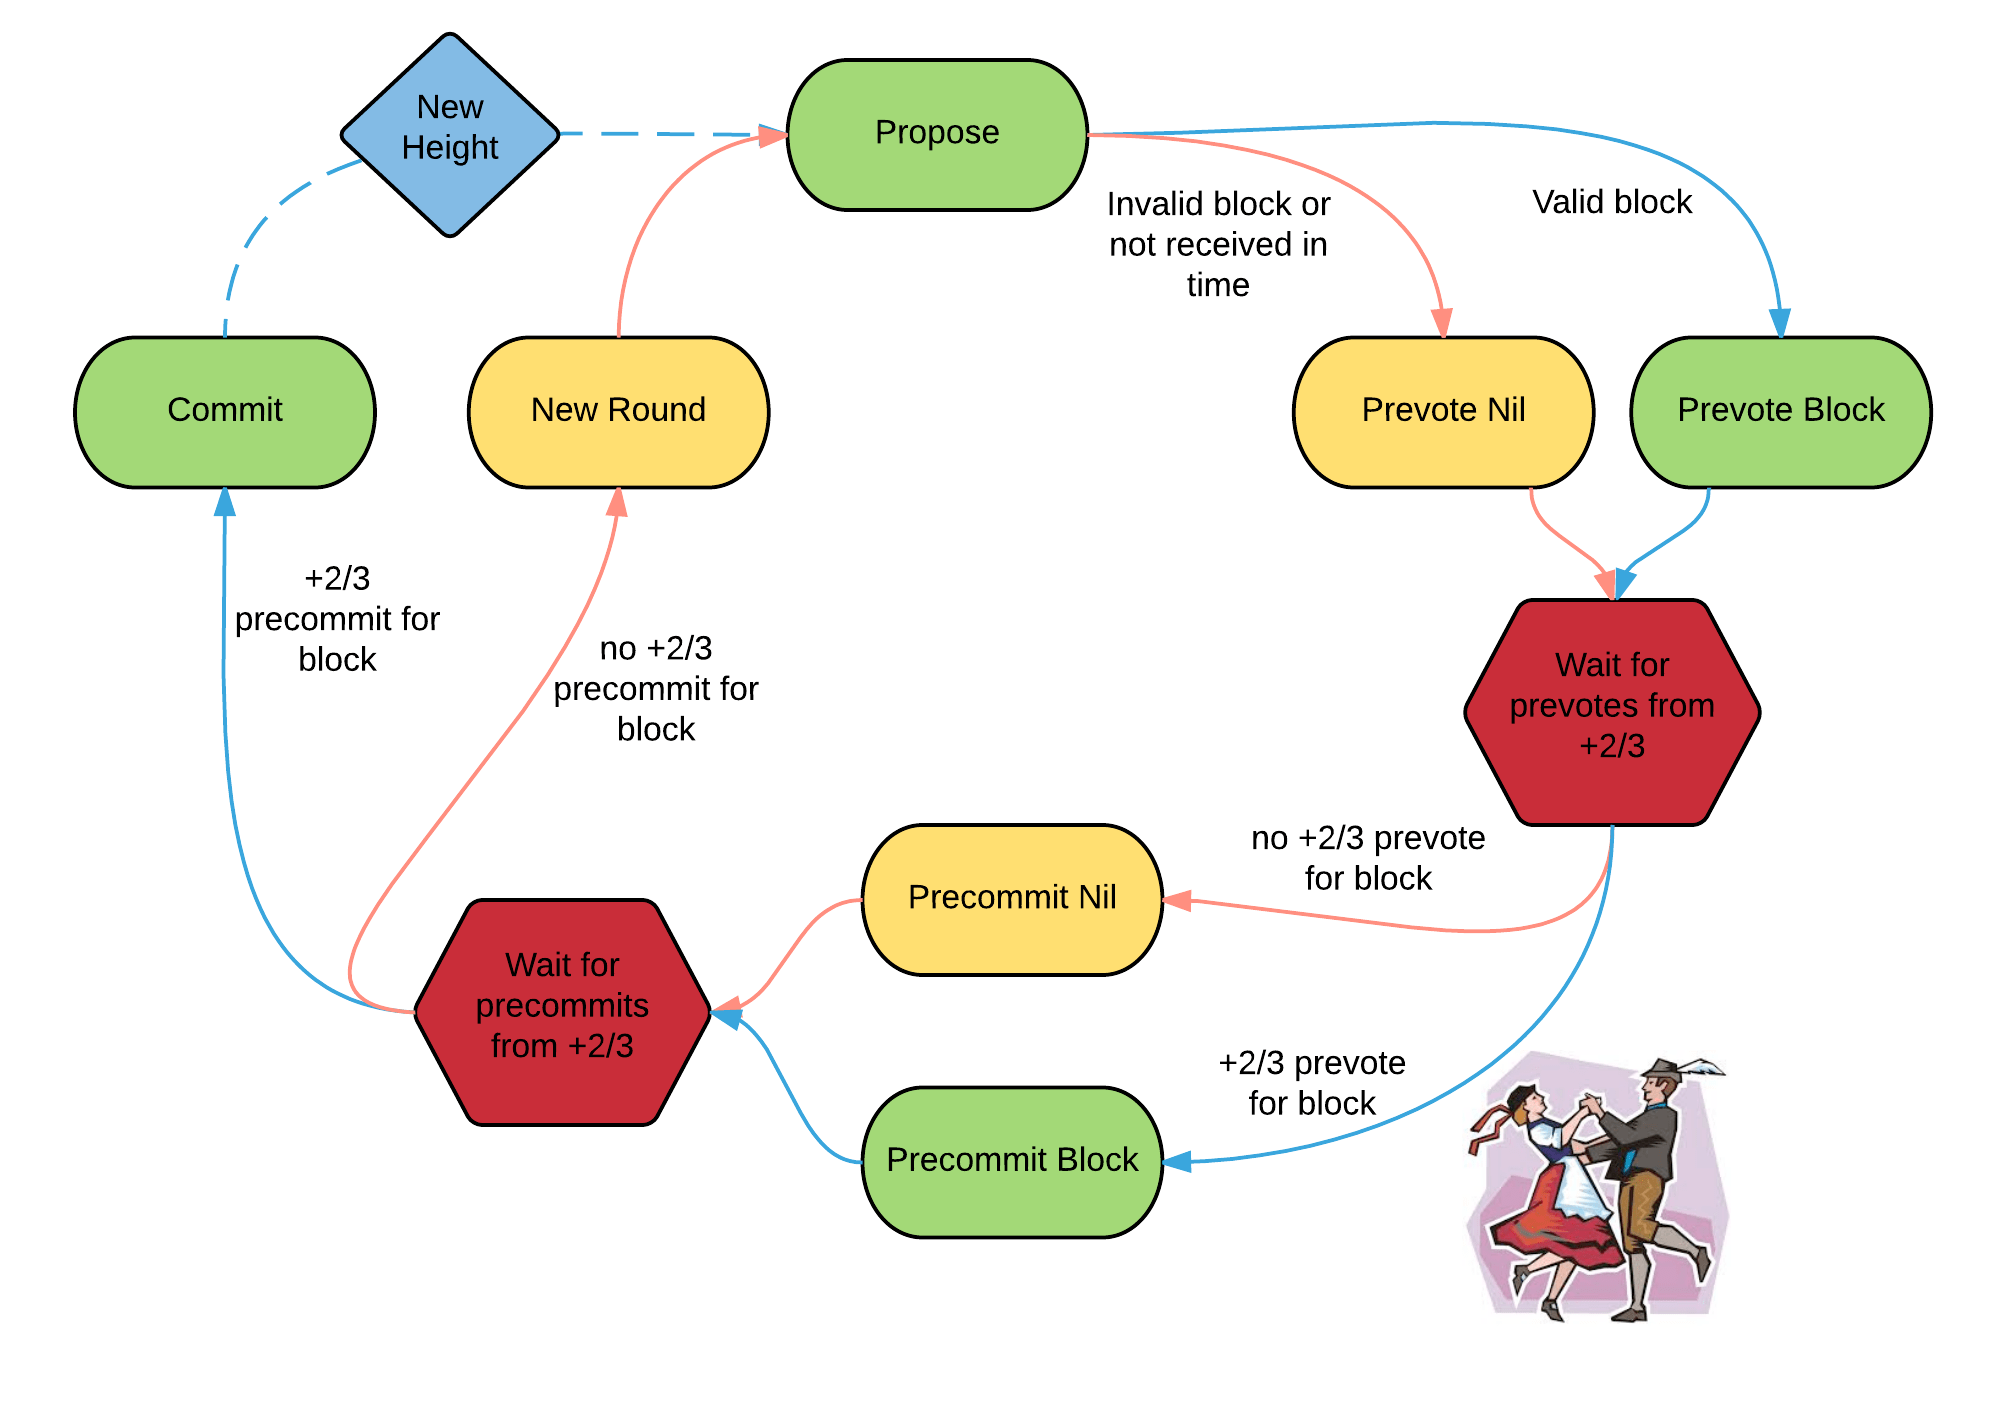
\includegraphics[width=\textwidth]{figures/cometbft.png}
    \caption{Consensus Overview CometBFT Source\cite{cometbft-overview}}
    \label{fig:cometbft-overview}
\end{figure}


\subsection{ABCI}
The \gls{abci} interface is a set of standard protocols that defines the communication between the consensus engine and the application. By enabling the division of consensus engine logic from application logic, it facilitates the development of applications on top of the Cosmos SDK.

The consensus engine and the application can communicate with one another without having to be aware of each other's internal workings thanks to the \gls{abci} interface, which serves as a mediator between them as shown in Lst \ref{lst:ABCI}. The development process is more flexible thanks to this separation of concerns as developers can focus on developing their particular application logic without worrying about the underlying consensus engine. Additionally, because the \gls{abci} interface offers a standardised method for the consensus engine to connect with the application, it facilitates interoperability between various blockchains that make use of the Cosmos SDK.

\newpage
\begin{lstlisting}[language=bash, caption=ABCI Interface. Source:\cite{app-based-blockchain},label={lst:ABCI}]
                      +---------------------+
                      |                     |
                      |     Application     |
                      |                     |
                      +--------+---+--------+
                               ^   |
                               |   | ABCI
                               |   v
                      +--------+---+--------+
                      |                     |
                      |                     |
                      |       CometBFT      |
                      |                     |
                      |                     |
                      +---------------------+
\end{lstlisting}


\section{Applications Architecture}
\label{ch:applicatoins-architecture}

So far this in this chapter we have seen a general overview on how the Cosmos SDK works and why its modular decoupled architecture helps developers when creating their applications. Thanks to CometBFT, developers can focus on the application's logic without having to worry about the uderlaying consensus and communication process of the state machine. In this subsection we will dissect how the application layer of our architecture works.

In fact, the application layer works in a very simple and modular way thanks to the Cosmos SDK. The framework provides us with a simple boilerplate implementation called baseApp. This baseApp implements the necessary methods to route the transactions to the different modules and also implements the \gls{abci} methods to communicate with the cometBTF engine. Modules can be viewed as small state machines within the state machine. They generally define a subset of the state, as well as a subset of message types. These messages are routed by the BaseApp and the module parses them using protobuf definitions. This is how byte transactions handled by the cometBFT are translated into the application logic.

On top of this core, the Cosmos SDK enables developers to build custom modules that implement the business logic of their application. In other words, while the core handles wiring and permits module composition, SDK custom made modules implement the majority of the application's functionality. Fig \ref{fig:application-modules} shows the general architecture of the application layer.

\begin{figure}[H]
    \centering
    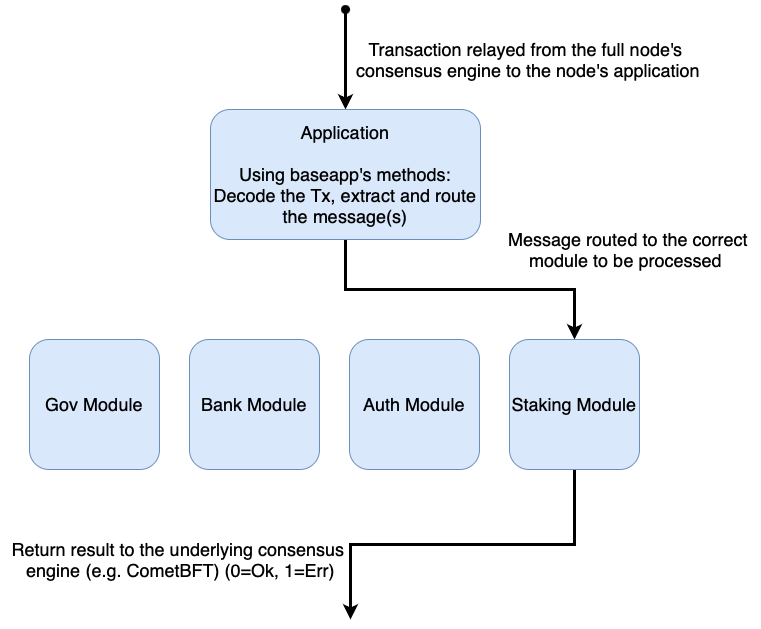
\includegraphics[width=\textwidth]{figures/prueba.png}
    \caption{Application architecture}
    \label{fig:application-modules}
\end{figure}

\chapter{Comparison of Consensus Mechanisms in the Cosmos SDK}
\label{ch:compare}

Consensus algorithms are the backbone of blockchain technology, ensuring that all participants in a network agree on the current state of the ledger. The Cosmos SDK, with its unique approach to blockchain architecture, utilizes various consensus mechanisms, each tailored for specific needs and scenarios. This chapter compares the consensus mechanisms available in the Cosmos SDK to those in other blockchain systems, like Hyperledger, Ethereum, and Bitcoin. We will evaluate their functionality, security, scalability, and decentralization, and discuss their relevance and application within the Cosmos SDK framework.

Understanding the right consensus mechanism for a blockchain application is critical, as it directly impacts the network's performance, security, and overall functionality. In the Cosmos SDK context, this choice influences not just the network's efficiency but also its integration capabilities and future scalability. Therefore, this chapter aims to provide a deeper understanding of these mechanisms and their practical implications in the Cosmos SDK environment.

\section{Types of Consensus Mechanisms}

Different consensus mechanisms offer varied approaches to achieve network agreement, each with distinct efficiency and security profiles. The Cosmos SDK, known for its flexibility and modularity, supports various types of consensus mechanisms, each suitable for different kinds of blockchain applications.

\subsection{Proof of Work (PoW)}

\gls{pow}, pioneered by Bitcoin, is a consensus mechanism where network participants, or miners, compete to solve cryptographic puzzles. This process validates transactions and adds new blocks to the blockchain, with successful miners receiving cryptocurrency rewards~\cite{nakamoto2008bitcoin}.

While \gls{pow} is known for its robust security, it is not the primary consensus mechanism in the Cosmos SDK due to its high energy consumption and slower transaction processing times. The Cosmos SDK favors more efficient and scalable consensus mechanisms, aligning with its goal of creating interconnected, high-performance blockchain networks.

\subsection{Proof of Stake (PoS)}

\gls{pos} is a consensus algorithm where the probability of validating transactions and creating new blocks is proportional to a participant's stake in the network. Unlike \gls{pow}, it does not require extensive computational power, making it more energy-efficient and suitable for scalable networks~\cite{king2012ppcoin}.

The Cosmos SDK leverages variants of \gls{pos}, optimizing it for better performance and reduced energy consumption. This adaptation aligns with the SDK's emphasis on creating scalable and efficient blockchain networks.

\subsection{Delegated Proof of Stake (DPoS)}

\gls{dpos}, an evolution of \gls{pos}, allows token holders to elect delegates to validate transactions and maintain the blockchain. This mechanism is known for its high transaction throughput and efficiency~\cite{larimer2014delegated}.

The Cosmos SDK, with its modular design, can incorporate \gls{dpos} in its ecosystem, providing an efficient and scalable consensus option for networks that require fast transaction processing and high throughput.

\subsection{Practical Byzantine Fault Tolerance (PBFT)}

\gls{pbft} is designed for distributed systems and focuses on achieving consensus even in the presence of malicious nodes. The Cosmos SDK's version of PBFT, known as Tendermint Core, is a cornerstone of its architecture, offering a balance of efficiency, security, and scalability~\cite{castro1999practical}.

\subsection{Directed Acyclic Graph (DAG)}

Although not a primary feature of the Cosmos SDK, \gls{dag} represents an innovative approach to consensus mechanisms, focusing on scalability and efficiency. As the Cosmos SDK continues to evolve, integrating \gls{dag} or similar mechanisms could enhance its capabilities in handling high-throughput and low-latency networks~\cite{lewenberg2015inclusive}.

\section{Conclusion}

Throughout this chapter, we have examined and compared various consensus mechanisms, highlighting their unique characteristics, strengths, and limitations. The Cosmos SDK, with its versatile and modular architecture, supports a range of consensus mechanisms, each designed to cater to specific requirements and scenarios in blockchain applications.

While the Cosmos SDK primarily utilizes Tendermint Core, a variant of \gls{pbft}, for its consensus needs, understanding the broader spectrum of consensus mechanisms like \gls{pow}, \gls{pos}, \gls{dpos}, and \gls{dag} is crucial. These mechanisms collectively represent the diverse approaches to achieving network consensus, each balancing aspects of security, efficiency, and scalability.

For the sake of simplicity and practicality, this thesis does not delve into modifying the default consensus mechanism provided by the Cosmos SDK. Instead, our focus is on leveraging the inherent strengths of Tendermint Core within the Cosmos SDK framework. This approach aligns with the goal of creating interconnected, efficient, and secure blockchain networks, which are fundamental to the Cosmos SDK's design philosophy.

In summary, the Cosmos SDK's adoption of Tendermint Core, complemented by its support for various other consensus mechanisms, demonstrates its commitment to providing a robust, efficient, and scalable foundation for blockchain development. This makes the Cosmos SDK a compelling choice for developers and organizations looking to build advanced blockchain solutions that require a balance of performance, security, and interoperability.


\chapter{Methodology}
\label{mt:methodology}

In this section, we will walk through all the organizational aspects related to the project: configuration management and \gls{cicd} workflows.

\section{Configuration Management}

Configuration management can be defined as a process that ensures the consistency and quality of a project/product through its life cycle and the various changes it undergoes. Sometimes the term is mistaken for version control, but in fact configuration management includes version control~\cite{hammond2012version}.

In this subsection we will talk about the different technologies and tools that have been used in order to keep a decent control of configuration management.

\subsection{Git \& GitHub}

As mentioned above, version control is a part of configuration management and is responsible for recognizing and managing the various changes of software code. Version control systems are software tools that help teams manage changes to source code over time. 

For this project Git has been the clear option since it is the market leader due to its huge speed and its branch and merge functionality, among others. Taken from its website \enquote{Git is a free and open source distributed version control system designed to handle everything from small to very large projects with speed and efficiency}.

GitHub is essentially a remote repository hosting platform for Git. It allows developers to work together on the same project from anywhere~\cite{chacon2014pro}.

\subsection{Git Workflow}

A Git workflow is a template for how to use git to accomplish work in a consistent and productive manner. Git is extremely flexible when it comes to managing changes, so there is no imposed or standardized process. When working with a team on a project, it is important to make sure that the entire team is familiar with how changes will be applied. 

Gitflow has been chosen for this project because of its versatility and the ability to generate branches for each of the features needed for the project, Figure~\ref{fig:gitflow-example}. In our case, it will be extremely useful to be able to develop each of the modules/micro-services of the system in parallel~\cite{driessen2010successful}.

\begin{figure}[H]
    \centering
    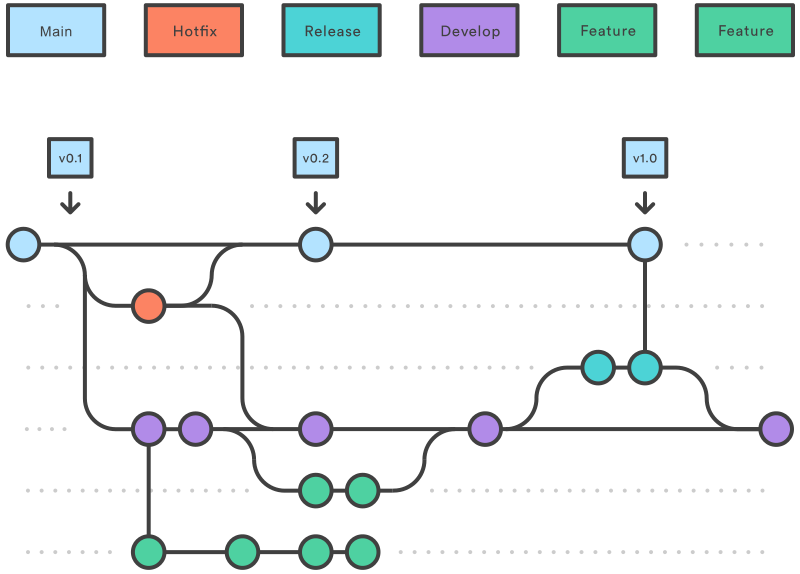
\includegraphics[width=0.55\textwidth]{figures/gitflow.png}
    \caption{Gitflow Scheme, Source: www.atlassian.com}
    \label{fig:gitflow-example}
\end{figure}

\section{CI/CD Workflows}

One of the main goals during the design phase of this thesis is to have a high level of automation to be able to maintain all the different development processes. Luckily GitHub provides us with a powerful tool for creating custom workflow pipelines, called GitHub actions. These workflows must be located in a folder called \textbf{.github/workflows}, in the root of the repository in different "YAML" files~\cite{github2020actions}.

GitHub actions fees depend on computing time and the runner's \gls{os}. Runners are responsible for executing the different jobs specified in a workflow, Tab~\ref{tab:action-fees} shows the different prices.

\begin{table}[h]
\centering
\caption{Runner Fees}
\label{tab:action-fees}
\begin{tabular}{@{}ll@{}}
\toprule
Linux             & \$0.008/min \\ \midrule
Windows           & \$0.016/min \\ \midrule
macOs             & \$0.08/min  \\ \midrule
Self-hosted       & Free        \\ \midrule
Public repository & Free       
\end{tabular}
\end{table}

\newpage
\subsection{Self-hosted Runner}

\begin{lstlisting}[language=bash, caption=Set up Self-hosted Runner,label={lst:self-hosted-runner}]
$ curl -o actions-runner-linux-x64-2.287.1.tar.gz -L https://github.com/actions/runner/releases/download/v2.287.1/actions-runner-linux-x64-2.287.1.tar.gz
$ tar xzf ./actions-runner-linux-x64-2.287.1.tar.gz
$ ./config.sh --url https://github.com/username/repository --token "YOUR TOKEN"
$ ./run.sh
$ sudo ./svc.sh install #this will create a systemd daemon to start the runner on start up
\end{lstlisting}

Self-hosted runners offer more control of hardware, \gls{os}, and software tools than GitHub-hosted runners provide. With self-hosted runners, you can choose to create a custom hardware configuration with more processing power or memory to run larger jobs, install software available on your local network, and choose an \gls{os} not offered by GitHub-hosted runners. Self-hosted runners can be physical, virtual, in a container, on-premises, or in a cloud.

To add a self-hosted runner, is as simple as going to the actions section in the repository settings and follow the instructions, Listing~\ref{lst:self-hosted-runner} shows the steps used to configure a Linux based runner for the project. From now on, our self-hosted runner will listen for jobs from our GitHub repository and start executing them whenever a workflow is triggered.

\subsection{Workflow Definition}

Two of the most important aspects to take into consideration when defining a workflow, are the branches or events that will trigger it and the jobs and tasks to be executed. Note that these jobs do not necessarily have to be sequentially executed, in fact they run in parallel by default. Nonetheless, GitHub actions allows us to establish dependencies between jobs, so that certain ones are executed before others.

Triggering events must be defined under the \enquote{on}: tag. Listing~\ref{lst:trigger-options} shows an example of a couple of interesting ones, for more information about triggering events follow the instructions in the action's documentation.

\begin{lstlisting}[caption=Common Workflow Triggers,label={lst:trigger-options}]
on:
  push:
    branches: [only when specific branches are pushed]
    branches-ignore: [ignored branches]
    paths: # triggers when a push to specific files occurs
        - '**.go'
  pull_request:
    types: [pull request activity type]
  workflow_dispatch: # allows the workflow to be triggered manually
\end{lstlisting}

As for the job definition, they all must be declared under the \enquote{job} tag. Jobs run in parallel by default as we explained before. To run them sequentially, you can define dependencies as Listing~\ref{lst:jobs-definition} shows. Also, the runner which will execute the job, needs to be chosen in the definition.

\begin{lstlisting}[caption=Job Dependencies Definition,label={lst:jobs-definition}]
jobs:
  jobA:
    runs-on: [self-hosted] # the job will be forwarded to our self-hosted runner
  jobB:
    runs-on: [ubuntu-latest] # the job will be executed in a hosted ubuntu machine
    needs: jobA
  jobC:
    runs-on: [self-hosted]
    if: ${{ always() }} #jobC will execute regardless of jobA & jobB output
    needs: [jobA, jobB]
\end{lstlisting}

The most powerful feature about GitHub actions is the integration with its whole ecosystem. So for instance, each job has a list of steps which are always executed sequentially and they all need to pass, in order for the job to successfully finish. These task can be either manually specified or reused from the Action's marketplace, where everyone can either upload or reuse published actions. To use any of them, is as simple as specifying the dependency \enquote{publisher/actions@version}. Listing~\ref{lst:step-definition} shows an example of a reused action from the marketplace.

Another useful feature is the \enquote{secrets} environment, which lets you define repository level environment variables that need to be off the code, i.e, \gls{api} keys, tokens or cryptography private keys.

\begin{lstlisting}[caption=Steps Definition,label={lst:step-definition}]
steps:
- uses: actions/first-interaction@v1 # dependency definition
  with:
    repo-token: ${{ secrets.GITHUB_TOKEN }} # GitHub environment variable
    issue-message: 'message that will be displayed on users' first issue'
    pr-message: 'message that will be displayed on users' first pr'
\end{lstlisting}

\section{Application to Our Use Case}
\label{sec:application-use-case}

This section delineates how the methodologies discussed in this chapter are applied to our specific use case, which involves the development and deployment of blockchain nodes on \gls{aws}, managed and automated through GitHub actions. The aim is to elucidate the practical application of configuration management and \gls{cicd} workflows in the context of a blockchain-based project, ensuring a seamless and efficient development lifecycle.

\subsection{Architecture Overview}

The architecture of our project is designed to optimize performance, security, and scalability. The blockchain nodes, the backbone of our application, are hosted on \gls{aws}, providing robust and scalable cloud infrastructure. The codebase for the project resides on GitHub, which acts as the central repository for version control and collaboration among the development team.

To visualize the integration and interaction between different components of our project, an architecture diagram is essential. Figure~\ref{fig:architecture-diagram} illustrates the overall architecture, focusing on high availability and high scalability of the service thanks to the \gls{alb} which supports the \gls{grpc} protocol natively.

\begin{figure}[H]
    \centering
    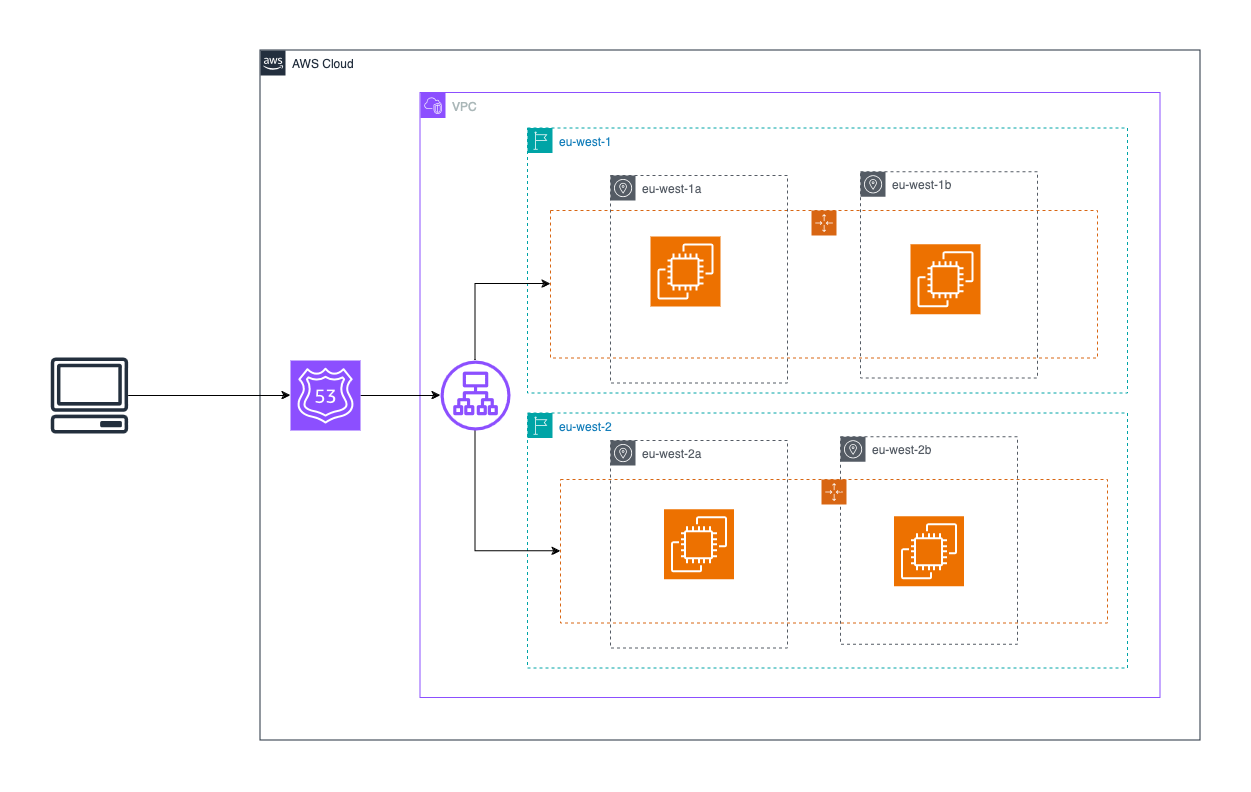
\includegraphics[width=\textwidth]{figures/aws.png}
    \caption{Overall Architecture Diagram}
    \label{fig:architecture-diagram}
\end{figure}

\newpage
\subsection{Deployment Sequence}
The deployment workflow is a critical aspect of our project, ensuring that the latest codebase changes are automatically tested, built, and deployed to the AWS environment. This process is facilitated by GitHub Actions, which automates the workflow based on specific triggers, such as a push to the main branch or a pull request.

A detailed diagram of the deployment workflow helps in understanding the sequence of events from code commit to deployment. Figure~\ref{fig:deployment-workflow-diagram} depicts this workflow, including the steps taken by GitHub Actions to deploy the application onto \gls{aws}.

\begin{figure}[H]
    \centering
    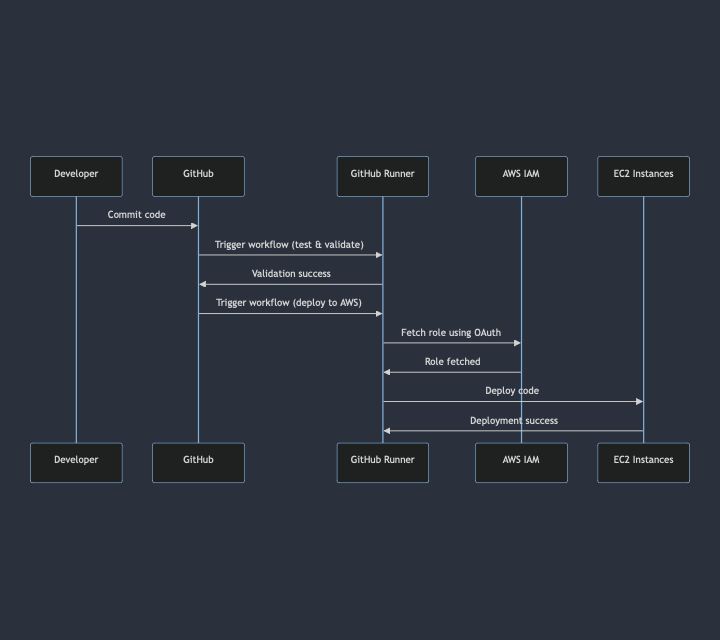
\includegraphics[width=\textwidth]{figures/sequence.png}
    \caption{Deployment Workflow Diagram}
    \label{fig:deployment-workflow-diagram}
\end{figure}

\subsection{Implementation Details}
The implementation of our use case begins with committing code changes to the GitHub repository. These changes trigger predefined GitHub Actions workflows.

The workflows include various jobs, such as linting, testing, building, and deploying. Each job is executed in an environment specified by the workflow, with most deployment tasks directed to self-hosted runners equipped to interact with \gls{aws} services. These runners use the OAuth protocol to authenticate against \gls{iam} in \gls{aws}, ensuring that the deployment process is both secure and efficient.

Upon successful completion of the deployment job, the updated application is live, ready to be accessed by users. This automated workflow not only minimizes human error but also significantly accelerates the development lifecycle, allowing for rapid iteration and feedback.

In conclusion, the application of configuration management and \gls{cicd} workflows to our use case exemplifies a modern, efficient, and scalable approach to software development and deployment. By leveraging industry-standard tools and practices, we ensure that our blockchain project remains at the forefront of technological advancements.

\chapter{Case Study: Private Blockchain for Crowdfunding}

In this case study, we explore the implementation of a private blockchain for crowdfunding using the Cosmos SDK. This approach is particularly relevant in the current technological landscape, where blockchain technology significantly impacts various industries, offering innovative paradigms for secure, decentralized transactions and data management. Crowdfunding, a popular method for raising capital, stands to benefit greatly from the advantages offered by blockchain technology, such as enhanced transparency, security, and efficiency.

\subsection{Relevance and Objectives}

The objectives of this case study are as follows:
\begin{itemize}
    \item To demonstrate the practical application of blockchain technology in a crowdfunding context, underscoring the advantages over traditional methods.
    \item To delve into the specific features and capabilities of the Cosmos SDK in constructing a customized, efficient, and secure private blockchain.
    \item To provide a comprehensive guide and framework for developers and entrepreneurs aiming to utilize blockchain technology in crowdfunding or related fields.
\end{itemize}

This case study seeks to bridge theoretical concepts with practical application, offering a tangible example of how blockchain technology can be applied innovatively in real-world scenarios.
\subsection{Cosmos SDK in Crowdfunding}

Crowdfunding represents a unique application for blockchain technology, where the principles of decentralization, transparency, and security are paramount. Utilizing the Cosmos SDK for a private blockchain in a crowdfunding context offers several distinct advantages:

\begin{itemize}
    \item \textbf{Modularity:} The Cosmos SDK's modular structure enables the development of specialized functionalities tailored to crowdfunding needs. Modules for project listings, investor interactions, and fund management can be created, providing a comprehensive ecosystem for crowdfunding activities.
    \item \textbf{Interoperability:} A key feature of the Cosmos SDK is its ability to facilitate interoperability between different blockchain networks. This feature is crucial for a crowdfunding platform, as it allows the integration of diverse assets and broadens the scope for investments and investor participation.
    \item \textbf{Scalability:} The Cosmos SDK is designed to support scalable applications, which is essential for crowdfunding platforms expecting a high volume of transactions and interactions. Its underlying consensus mechanisms, such as Tendermint BFT, ensure that the platform can handle growth efficiently without compromising performance.
    \item \textbf{Customizability:} The SDK's flexible architecture allows for the creation of a customized user experience and specific features that cater to the unique requirements of crowdfunding, such as project validation, funding stages, and return distributions.
    \item \textbf{Security:} Ensuring the security of funds and transactions is critical in crowdfunding. The Cosmos SDK's security model, which includes features like role-based permissions and secure transaction handling, provides a robust foundation for building a trustworthy crowdfunding platform.
\end{itemize}

In the following sections, we will explore the implementation aspects of a crowdfunding platform using the Cosmos SDK, focusing on the design, development, and operation of key features in line with the requirements of crowdfunding activities.

\subsubsection{Project Setup and State Modeling}

The initial phase in developing a crowdfunding platform with the Cosmos SDK involves setting up the project structure and modeling the state. This process lays the foundation for how the blockchain will manage and store data related to crowdfunding activities.

\paragraph{Defining the Data Model}

In a crowdfunding context, the state of the blockchain must accurately represent the dynamic relationships and activities between various entities such as projects, investors, and funding stages. The Cosmos SDK's flexibility in defining the data model is crucial for capturing the multifaceted nature of crowdfunding projects. This flexibility allows for the creation of tailored entities that reflect the specific needs and structures inherent in crowdfunding platforms.

For instance, the `Project` entity encapsulates essential information about each crowdfunding initiative, including its identification, sponsorship details, financial targets, and current status. This comprehensive representation is crucial for tracking the progress and managing the lifecycle of crowdfunding projects.

The `Investor` entity models the stakeholders in a project, detailing their investment contributions and accrued benefits. By defining this entity, the platform can effectively manage investor relations, equity distribution, and profit sharing, which are core aspects of crowdfunding dynamics.

The `Stage` entity reflects the phased approach common in crowdfunding projects, where each stage represents a milestone or a specific funding goal. This modular approach to project development and funding allows for more granular management and tracking of the project's progress.

\begin{lstlisting}[language=go, caption={Protobuf Definitions for Project, Investor, and Stage}, label=lst:protobuf-definitions]
message Project {
  uint64 id = 1;
  string sponsor = 2;
  cosmos.base.v1beta1.Coin target = 3 [(gogoproto.nullable) = false];
  cosmos.base.v1beta1.Coin current = 4 [(gogoproto.nullable) = false];
  string state = 5;
  repeated Investor investors = 6;
  repeated Stage stages = 7;
}

message Investor {
  string address = 1;
  cosmos.base.v1beta1.Coin equity = 2 [(gogoproto.nullable) = false];
  int64 profit = 3;
}

message Stage {
  string name = 1;
  cosmos.base.v1beta1.Coin allocation = 2 [(gogoproto.nullable) = false];
}
\end{lstlisting}


By leveraging Protobuf for defining these data structures, the Cosmos SDK ensures consistency, efficiency, and the ability to evolve the data model as the platform grows. This approach not only enhances the blockchain's data integrity but also ensures that it can adapt to the changing needs of crowdfunding activities.

\paragraph{State Management}

State management is a core aspect of any blockchain application. In the context of crowdfunding, the state represents the current condition of all projects, investments, and transactions on the platform. The Cosmos SDK's multistore structure allows each module to manage its part of the state, leading to enhanced modularity and maintainability.

A critical element in the state management system of the Cosmos SDK is the concept of the 'keeper'. In each module, the keeper acts as a guardian or manager of the module's state, as shown in Img~\ref{fig:application-multistore}. It is responsible for interfacing with the module's Key-Value store (KVStore), a datastore that holds the state of the module. The keeper, through a set of predefined APIs, provides a secure and controlled access to the KVStore, ensuring that only authorized operations can be performed on the module's state.

The keeper's role is multifaceted:

\begin{itemize}
    \item \textbf{Access Control:} It enforces access control, determining which parts of the state can be accessed or modified by other modules.
    \item \textbf{Data Encapsulation:} The keeper helps in encapsulating the internal state of a module, exposing only necessary information to other modules, thereby maintaining data integrity and security.
    \item \textbf{State Interaction:} It facilitates interactions with the state, such as querying, updating, or deleting records related to the crowdfunding projects and investments.
\end{itemize}

In essence, the keeper in Cosmos modules plays a vital role in state management by safeguarding the keys to access the KVStore. This mechanism not only secures the data but also aligns with the modular architecture of the Cosmos SDK, where each module operates as an independent yet integral part of the overall application, maintaining its distinct state and logic.

\begin{figure}[H]
    \centering
    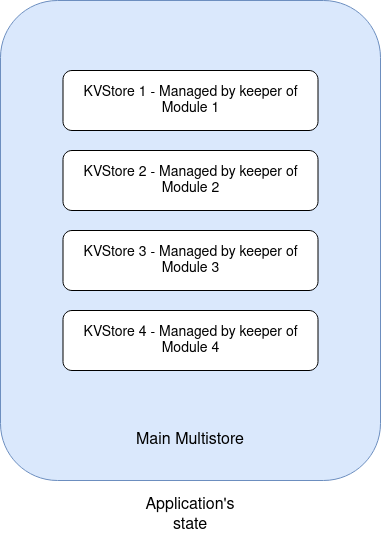
\includegraphics[scale=0.45]{figures/multistore.png}
    \caption{Application's state}
    \label{fig:application-multistore}
\end{figure}

\paragraph{Transaction Handling}

Transactions in the crowdfunding platform are actions that change the state, such as creating a new project, investing in a project, or distributing funds. Each transaction type is defined with its validation logic, ensuring that only valid changes are applied to the state. The Cosmos SDK facilitates the creation of these transactions, handling the lifecycle from initiation to inclusion in the blockchain.

\paragraph{Query System}

A robust query system is essential for a crowdfunding platform, enabling users to retrieve information about projects and investments. The Cosmos SDK supports a flexible query interface, allowing users to interact with the blockchain's state efficiently. Queries can be made for specific projects, funding stages, and investment details, providing transparency and accessibility to platform participants.

In the next sections, we delve deeper into the implementation of these components, illustrating how the Cosmos SDK is utilized to build a comprehensive crowdfunding solution.

\section{Transaction Types and Their Implementation}

In a crowdfunding platform developed with the Cosmos SDK, transactions play a pivotal role in facilitating various operations and interactions within the ecosystem. These transactions represent different actions that can be performed by users, such as creating new projects, investing in projects, or distributing returns. This section delves into the types of transactions that are fundamental to the crowdfunding platform and their implementation using the Cosmos SDK.

\subsection{Defining Transaction Types}

The Cosmos SDK allows for the definition of custom transaction types to suit specific application needs. In the context of a crowdfunding platform, several transaction types are essential:

\begin{itemize}
    \item \textbf{CreateProject:} Initiates the creation of a new crowdfunding project, specifying details like project sponsor, funding target, and project stages.
    \item \textbf{InvestorBuyIn:} Enables investors to contribute funds to a project, marking their stake in the crowdfunding venture.
    \item \textbf{ChangeState:} Alters the state of a project, such as moving it from active to funded, or from funded to completed.
    \item \textbf{MoneyIn \& MoneyOut:} Manages the flow of funds into and out of the project, ensuring proper allocation and distribution.
    \item \textbf{SponsorCancel \& SponsorAccept:} Used by project sponsors to either cancel a project in its early stages or accept funding upon reaching the target.
    \item \textbf{AdminAdd \& AdminDelete:} Administering the platform by adding or removing administrators or project managers.
    \item \textbf{NextStage:} Progresses the project through its different stages, ensuring milestones are met before proceeding.
    \item \textbf{ShareProfit:} Distributes profits or returns to investors based on their contributions once the project generates revenue.
    \item \textbf{UpdateDraftProject:} Modifies details of a project that is still in its draft phase.
\end{itemize}

Each of these transaction types is implemented as a specific \gls{grpc} endpoint, as shown in Listing \ref{lst:gRPC-endpoints}. This structure not only brings clarity to the various operations possible within the crowdfunding platform but also ensures that each transaction is handled efficiently and securely within the Cosmos SDK framework.

The combination of well-defined transactions and efficient gRPC endpoints enables the crowdfunding platform to function seamlessly, providing a robust and user-friendly experience for both project creators and investors. This approach exemplifies the Cosmos SDK's versatility in handling diverse transaction types, a critical aspect for the success of any blockchain-based application.

\begin{lstlisting}[language=go, caption=gRPC endpoints definition,label={lst:gRPC-endpoints}]
service Msg {
  rpc CreateProject(MsgCreateProject) returns (MsgCreateProjectResponse);
  rpc InvestorBuyIn(MsgInvestorBuyIn) returns (MsgInvestorBuyInResponse);
  rpc ChangeState(MsgChangeState) returns (MsgChangeStateResponse);
  rpc MoneyIn(MsgMoneyIn) returns (MsgMoneyInResponse);
  rpc MoneyOut(MsgMoneyOut) returns (MsgMoneyOutResponse);
  rpc SponsorCancel(MsgSponsorCancel) returns (MsgSponsorCancelResponse);
  rpc SponsorAccept(MsgSponsorAccept) returns (MsgSponsorAcceptResponse);
  rpc AdminAdd(MsgAdminAdd) returns (MsgAdminAddResponse);
  rpc AdminDelete(MsgAdminDelete) returns (MsgAdminDeleteResponse);
  rpc NextStage(MsgNextStage) returns (MsgNextStageResponse);
  rpc ShareProfit(MsgShareProfit) returns (MsgShareProfitResponse);
  rpc UpdateDraftProject(MsgUpdateDraftProject) returns (MsgUpdateDraftProjectResponse);
}
\end{lstlisting}

\subsubsection{General Process for Implementing Transactions in Cosmos SDK}

The Cosmos SDK offers a structured approach to implementing transactions, which is crucial for maintaining the integrity and functionality of a blockchain application. The general process can be outlined in the following steps:

\begin{enumerate}
    \item \textbf{Defining the Transaction Message:}
    \begin{itemize}
        \item The first step is to define the transaction message using Protobuf. This involves specifying the structure of the data that will be included in the transaction. 
        \item The message should encompass all the necessary fields that are required to perform the transaction. This could include identifiers, amounts, addresses, or any other relevant information.
        \item The defined message acts as a blueprint for the transaction, ensuring that all necessary data is included and structured correctly for processing.
    \end{itemize}

    \item \textbf{Implementing the CLI Command:}
    \begin{itemize}
        \item Once the transaction message is defined, the next step is to implement the corresponding \gls{cli} command.
        \item This command allows users to interact with the blockchain application and execute transactions from the command line.
        \item The implementation involves coding the logic that will take user inputs, validate them, and construct the transaction message based on these inputs.
        \item The \gls{cli} command typically includes error handling and may have additional logic for transaction fees, signing, and broadcasting the transaction to the network.
    \end{itemize}
\newpage
    \item \textbf{Coding the Keeper Function:}
    \begin{itemize}
        \item The keeper function is responsible for updating the state of the blockchain based on the transaction.
        \item It involves writing the logic that will be executed when a transaction is processed. This includes validating the transaction, updating the state, and handling any side effects.
        \item The keeper function interacts with the blockchain's state machine, ensuring that the state changes are consistent and secure.
        \item It's crucial that the keeper function is thoroughly tested to ensure it handles all possible scenarios and edge cases correctly.
    \end{itemize}
\end{enumerate}

Following this structured process ensures that each transaction type is correctly implemented and integrated into the blockchain application. This methodology not only maintains the consistency and reliability of the application but also provides a clear framework for developing new transaction types as the application evolves.

In the following sections, we will be implementing different transaction, providing detailed insights into each step of the process for a comprehensive understanding.

\subsection{Implementation of the CreateProject Transaction}

The `CreateProject` transaction plays a pivotal role in the crowdfunding platform, enabling the initiation of new projects. Its implementation in the Cosmos SDK involves a series of well-defined steps, each contributing to the robust functionality of the transaction. This section details the engineering process behind the `CreateProject` transaction.

\subsubsection{Defining the Protobuf Message}

The first step in implementing the `CreateProject` transaction is defining its structure using Protocol Buffers (Protobuf). Protobuf is a language-neutral, platform-neutral, extensible way of serializing structured data, making it ideal for this purpose.

\newpage
\begin{lstlisting}[language=go, caption=CreateProject protobuf definition, label={lst:create_project_proto}]
message MsgCreateProject {
  string                 sponsor = 1;
  cosmos.base.v1beta1.Coin target  = 2 [(gogoproto.nullable) = false];
  repeated Stage         stages  = 3;
}
\end{lstlisting}

The `MsgCreateProject` message encapsulates all necessary data for creating a project, such as the sponsor's name, target funding amount, and the project stages. Each field is carefully chosen to capture the essential attributes of a crowdfunding project.

\subsubsection{Implementing the CLI Command}

The next phase involves implementing the \gls{cli} command. This command facilitates interaction with the blockchain, allowing users to initiate a `CreateProject` transaction.

The \gls{cli} command, as shown is Lst~\ref{lst:create-project-cli-implementation}, provides a user-friendly way to submit the `CreateProject` transaction. It includes error checking and handles user inputs, converting them into the Protobuf message format.

\newpage
\begin{lstlisting}[language=go, caption=CreateProject CLI protobuf definition, label={lst:create-project-cli-implementation}]
func CmdCreateProject() *cobra.Command {
	cmd := &cobra.Command{
		Use:   "create-project [target] [stages]",
		Short: "Broadcast message create-project",
		Args:  cobra.ExactArgs(2),
		RunE: func(cmd *cobra.Command, args []string) (err error) {
			argTarget, err := sdk.ParseCoinNormalized(args[0])
			if err != nil {
				return err
			}
			argStages, err := types.ParseStageNormalized(args[1])
			if err != nil {
				return err
			}
			clientCtx, err := client.GetClientTxContext(cmd)
			if err != nil {
				return err
			}
			msg := types.NewMsgCreateProject(
				clientCtx.GetFromAddress().String(),
				argTarget,
				argStages,
			)
			if err := msg.ValidateBasic(); err != nil {
				return err
			}
			return tx.GenerateOrBroadcastTxCLI(clientCtx, cmd.Flags(), msg)
		},
	}
	flags.AddTxFlagsToCmd(cmd)
	return cmd
}
\end{lstlisting}

\subsubsection{Backend Processing}

Upon receiving a `CreateProject` transaction request, either through the \gls{cli} or a \gls{grpc} call, the Cosmos SDK's backend processes it. The transaction message is first validated, ensuring all required fields are provided and meet the necessary criteria.

\begin{verbatim}
$ daemonNamed tx appName create-project --sponsor "Project Sponsor" \
    --target "1000TOKENNAME" \
    --stages "Stage 1:100TOKENNAME,Stage 2:500TOKENNAME"
\end{verbatim}

This command, as illustrated, is an example of how users can initiate the `CreateProject` transaction using the Cosmos SDK CLI.

\subsubsection{Keeper Function Implementation}

The keeper function is where the transaction's logic is executed. This function updates the state of the blockchain with the new project's information.

\begin{lstlisting}[language=go, caption=Keeper implementation for CreateProject, label={lst:keeper_create_project}]
func (k msgServer) CreateProject(goCtx context.Context, msg *types.MsgCreateProject) (*types.MsgCreateProjectResponse, error) {
	ctx := sdk.UnwrapSDKContext(goCtx)
	var project = types.Project{
		Stages:  msg.Stages,
		Sponsor: msg.Sponsor,
		Target:  msg.Target,
	}
	id, err := k.AppendProject(
		ctx,
		project,
	)
	if err != nil {
		return &types.MsgCreateProjectResponse{}, err
	}
	types.EmitEvent(ctx, types.EventTypeProjectCreated, id, msg.Sponsor)
	return &types.MsgCreateProjectResponse{
		Id:      id,
		Address: msg.Sponsor,
	}, nil
}
\end{lstlisting}

The keeper function, as demonstrated, is responsible for appending the new project to the blockchain. It validates the transaction, checks for authorization, and updates the blockchain's state accordingly.

Following the successful creation of a project, an event is emitted. This event logs the creation, providing an auditable trail of the transaction. It includes details such as the project ID and sponsor's address.


\subsection{Updating Draft Projects}

Projects in the crowdfunding platform, upon their initial creation, are in a \texttt{draft} state. This status indicates that the project details are preliminary and subject to revisions. The \texttt{UpdateDraftProject} transaction plays a crucial role in this phase, allowing authorized users to modify essential project attributes like target funding and project stages.

\subsubsection{Protobuf Message for UpdateDraftProject}

The structure of the \texttt{UpdateDraftProject} transaction is defined using Protobuf, ensuring a consistent and efficient data representation.

\newpage
\begin{lstlisting}[language=go, caption=UpdateDraftProject protobuf definition, label={lst:update_draft_project_proto}]
message MsgUpdateDraftProject {
  string                                creator   = 1;
  uint64                                projectId = 2;
  cosmos.base.v1beta1.Coin              target    = 4 [(gogoproto.nullable) = false];
  repeated Stage                        stages    = 5;
}
\end{lstlisting}

This Protobuf message includes fields for the project's unique identifier, updated target funding, and revised stages, capturing the essential elements for updating a draft project.

\subsubsection{Authorizing Updates}

Modification of a project's details requires appropriate authorization. The \texttt{UpdateDraftProject} transaction ensures that only authorized individuals, typically the project sponsor, can make changes to the project in its draft state.

\subsubsection{Implementing the Keeper Function}

The keeper function is at the core of processing the \texttt{UpdateDraftProject} transaction. It validates the transaction, checks for authorization, and applies the updates to the project's state.

\begin{lstlisting}[language=go, caption=Keeper implementation for UpdateDraftProject, label={lst:keeper-update-draft}]
func (k msgServer) UpdateDraftProject(goCtx context.Context, msg *types.MsgUpdateDraftProject) (*types.MsgUpdateDraftProjectResponse, error) {
	ctx := sdk.UnwrapSDKContext(goCtx)
	projectId, err := k.updateDraftProjectInfo(ctx, msg.ProjectId, msg.Target, msg.Stages, msg.Creator)
	if err != nil {
		return nil, err
	}
	return &types.MsgUpdateDraftProjectResponse{
		ProjectId: projectId,
	}, nil
}
func (k Keeper) updateDraftProjectInfo(ctx sdk.Context, projectId uint64, target sdk.Coin, stages []*types.Stage, signer string) (uint64, error) {
	project, found := k.getProjectId(ctx, projectId)
	if !found {
		return 0, types.ErrProjectNotFound
	}
	if strings.Compare(signer, project.Sponsor) != 0 {
		return 0, types.ErrNotProjectSponsor
	}
	if strings.Compare(project.State, types.ProjectStateDraft) != 0 {
		return 0, types.ErrProjectNotDraft
	}
	if err := k.checkStages(stages, target); err != nil {
		return 0, err
	}
	project.Target = target
	project.Stages = stages
	k.saveProject(ctx, &project)
	return project.Id, nil
}
\end{lstlisting}

This keeper function checks if the project is in a draft state, validates the updates against the existing project structure, and then commits the changes to the blockchain.

\subsubsection{CLI Command for Updating Draft Projects}

To facilitate user interaction with the blockchain for updating projects, a \gls{cli} command is provided, simplifying the process of initiating the \texttt{UpdateDraftProject} transaction.

\newpage
\begin{lstlisting}[language=go, caption=Create Project CLI definition, label={lst:update-draft-cli}]
func CmdUpdateDraftProject() *cobra.Command {
	cmd := &cobra.Command{
		Use:   "update-draft-project [project-id] [target] [stages]",
		Short: "Broadcast message update-draft-project",
		Args:  cobra.ExactArgs(3),
		RunE: func(cmd *cobra.Command, args []string) (err error) {
			argProjectId, err := cast.ToUint64E(args[0])
			if err != nil {
				return err
			}
			argTarget, err := sdk.ParseCoinNormalized(args[1])
			if err != nil {
				return err
			}
			argStages, err := types.ParseStageNormalized(args[2])
			if err != nil {
				return err
			}
			clientCtx, err := client.GetClientTxContext(cmd)
			if err != nil {
				return err
			}
			msg := types.NewMsgUpdateDraftProject(
				clientCtx.GetFromAddress().String(),
				argProjectId,
				argTarget,
				argStages,
			)
			if err := msg.ValidateBasic(); err != nil {
				return err
			}
			return tx.GenerateOrBroadcastTxCLI(clientCtx, cmd.Flags(), msg)
		},
	}
	flags.AddTxFlagsToCmd(cmd)
	return cmd
}
\end{lstlisting}

This CLI command allows users to specify the project ID, updated target, and revised stages, streamlining the process of modifying a draft project.

\subsubsection{Executing the Transaction}

The execution of the \texttt{UpdateDraftProject} transaction can be done via the Cosmos SDK \gls{cli} or through a \gls{grpc} call. The CLI command example is as follows:

\begin{verbatim}
$ daemonNamed tx appName update-draft-project --project-id "idNumber" \
    --target "1000TOKENNAME" \
    --stages "Stage 1:100TOKENNAME,Stage 2:500TOKENNAME"
\end{verbatim}

This command line initiates the transaction, sending the updated project details to the blockchain for processing and validation.

The \texttt{UpdateDraftProject} transaction is an essential feature of the crowdfunding platform, offering flexibility and control during the project's initial development phase. It ensures that projects can evolve and refine their details before entering the active fundraising stage, thereby enhancing the platform's adaptability and responsiveness to changing needs and feedback.

\subsection{Investor Participation Transaction}

The \texttt{InvestorBuyIn} transaction is fundamental in the crowdfunding platform, enabling investors to financially contribute to projects of their interest. This transaction marks the investor's entry into the project, signifying their commitment and expectation of potential returns.

\subsubsection{Protobuf Message for InvestorBuyIn}

The transaction's structure is defined using Protobuf, which ensures a clear and efficient representation of the necessary data for an investor's participation.

\begin{lstlisting}[language=go, caption=InvestorBuyIn protobuf definition, label={lst:investor_buyin_proto}]
message MsgInvestorBuyIn {
  string                           investor = 1;
  uint64                           projectId = 2;
  cosmos.base.v1beta1.Coin         amount    = 3 [(gogoproto.nullable) = false];
}
\end{lstlisting}

This Protobuf message includes the investor's address, the project ID they wish to invest in, and the amount of their investment.

\subsubsection{Processing Investor Contributions}

Upon initiation of an \texttt{InvestorBuyIn} transaction, the platform processes the investor's contribution, ensuring that it adheres to the project's requirements and investment rules.

\subsubsection{Implementing the Keeper Function for InvestorBuyIn}

The keeper function is responsible for validating and processing the \texttt{InvestorBuyIn} transaction, updating the project's state with the new investment details.

\begin{lstlisting}[language=go, caption=Keeper implementation for Investor Buy-in, label={lst:keeper_investor_buyin}]
func (k msgServer) InvestorBuyIn(goCtx context.Context, msg *types.MsgInvestorBuyIn) (*types.MsgInvestorBuyInResponse, error) {
	ctx := sdk.UnwrapSDKContext(goCtx)
	var investor = types.Investor{
		Address: msg.Investor,
		Equity:  msg.Amount,
	}
	appendedAddr, err := k.AppendInvestorBuyIn(ctx, msg.ProjectId, investor)
	if err != nil {
		return &types.MsgInvestorBuyInResponse{}, err
	}
	return &types.MsgInvestorBuyInResponse{
		InvestorAddr: appendedAddr,
	}, nil
}

func (k Keeper) AppendInvestorBuyIn(ctx sdk.Context, id uint64, investor types.Investor) (string, error) {
	if investor.Equity.Amount.Equal(sdk.ZeroInt()) {
		return "", types.ErrCoinZeroAmount
	}
	project, found := k.getProjectId(ctx, id)
	if !found {
		return "", types.ErrProjectNotFound
	}
	if project.State != types.ProjectStateActive {
		return "", types.ErrProjectNotActive
	}
	if strings.Compare(project.Target.Denom, investor.Equity.Denom) != 0 {
		return "", types.ErrCoinDiffDenom
	}
	if project.Target.Sub(project.Current).IsLT(investor.Equity) {
		return "", types.ErrOverFunded
	}
	addr, err := sdk.AccAddressFromBech32(investor.Address)
	if err != nil {
		return "", err
	}
	if err := k.bankKeeper.SendCoinsFromAccountToModule(ctx, addr, types.ModuleName, sdk.NewCoins(investor.Equity)); err != nil {
		return "", err
	}
	project.Investors = appendInvestor(project.Investors, &investor)
	project.Current = project.Current.Add(investor.Equity)
	if project.Target.IsEqual(project.Current) {
		project.State = types.ProjectStatePending
		types.EmitEvent(ctx, types.EventTypeProjectPending, project.Id, investor.Address)
	} else {
		types.EmitEvent(ctx, types.EventTypeProjectInvested, project.Id, investor.Address)
	}
	k.saveProject(ctx, &project)
	return investor.Address, nil
}
\end{lstlisting}

This function ensures that the investment is correctly recorded and allocated to the specified project, updating the project's current funding status and the investor's stake.

\subsubsection{CLI Command for Investor Participation}

A \gls{cli} command is provided to facilitate the investor's interaction with the blockchain, enabling them to execute the \texttt{InvestorBuyIn} transaction seamlessly.

\begin{lstlisting}[language=go, caption=Investor Buy-in CLI Definition, label={lst:investor-buyin-cli}]
func CmdInvestorBuyIn() *cobra.Command {
	cmd := &cobra.Command{
		Use:   "investor-buy-in [project-id] [amount]",
		Short: "Broadcast message investor-buy-in",
		Args:  cobra.ExactArgs(2),
		RunE: func(cmd *cobra.Command, args []string) (err error) {
			argProjectId, err := cast.ToUint64E(args[0])
			if err != nil {
				return err
			}
			argAmount, err := sdk.ParseCoinNormalized(args[1])
			if err != nil {
				return err
			}
			clientCtx, err := client.GetClientTxContext(cmd)
			if err != nil {
				return err
			}
			msg := types.NewMsgInvestorBuyIn(
				clientCtx.GetFromAddress().String(),
				argProjectId,
				argAmount,
			)
			if err := msg.ValidateBasic(); err != nil {
				return err
			}
			return tx.GenerateOrBroadcastTxCLI(clientCtx, cmd.Flags(), msg)
		},
	}
	flags.AddTxFlagsToCmd(cmd)
	return cmd
}
\end{lstlisting}

Through this command, investors can specify the project they wish to invest in and the amount of their contribution, simplifying the investment process.

\subsubsection{Executing the InvestorBuyIn Transaction}

Investors can execute the \texttt{InvestorBuyIn} transaction via the Cosmos SDK \gls{cli} or through a gRPC request. The CLI command example is as follows:

\begin{verbatim}
$ daemonNamed tx appName investor-buy-in --project-id "projectId" \
    --amount "investmentAmount"
\end{verbatim}

This command facilitates the transaction process, marking the investor's financial entry into the selected project.

The \texttt{InvestorBuyIn} transaction plays a vital role in the crowdfunding ecosystem, enabling a direct and transparent channel for investors to support projects. It epitomizes the decentralized and participant-driven nature of blockchain-based crowdfunding, offering an efficient and secure mechanism for investment activities.

\subsection{Transitioning Project States}

The \texttt{ChangeState} transaction is essential for managing the lifecycle of crowdfunding projects, allowing administrators to update the state of a project at critical junctures.

The transition from the `draft` stage to the `active` stage marks the activation of a project on the private blockchain for crowdfunding. During the `active` stage, the project becomes open for investment, allowing investors to participate and contribute funds.

\subsubsection{Protobuf Message for ChangeState}

This transaction is defined using a Protobuf message, specifying the necessary details for altering the project's state.

The message includes the project ID, the desired new state, and the identity of the user initiating the change.

\begin{lstlisting}[language=go, caption=ChangeState protobuf definition, label={lst:change_state_proto_implementation}]
message MsgChangeState {
  string                        creator   = 1;
  uint64                        projectId = 2;
  string                        newState  = 3;
}
\end{lstlisting}

\subsubsection{Implementing the Keeper Function for ChangeState}

The keeper function ensures that the \texttt{ChangeState} transaction adheres to the platform's rules and correctly updates the project's status.

\begin{lstlisting}[language=go, caption=Keeper implementation for ChangeState, label={lst:keeper_change_state}]
func (k msgServer) ChangeState(goCtx context.Context, msg *types.MsgChangeState) (*types.MsgChangeStateResponse, error) {
	ctx := sdk.UnwrapSDKContext(goCtx)
	if !k.IsAdminAccount(ctx, msg.Creator) {
		return nil, types.ErrNotAdminAccount
	}
	projectId, err := k.changeProjectState(ctx, msg.NewState, msg.ProjectId)
	if err != nil {
		return &types.MsgChangeStateResponse{}, err
	}
	return &types.MsgChangeStateResponse{
		ProjectId: projectId,
	}, nil
}
\end{lstlisting}

This function validates the transaction, checks the authority of the initiator, and applies the state change to the project.

\subsubsection{CLI Command for Project State Transition}

A \gls{cli} command is provided for users to conveniently execute the \texttt{ChangeState} transaction.

\begin{lstlisting}[language=go, caption=Change State CLI Definition, label={lst:change-state-cli}]
func CmdChangeState() *cobra.Command {
	cmd := &cobra.Command{
		Use:   "change-state [project-id] [new-state]",
		Short: "Broadcast message change-state",
		Args:  cobra.ExactArgs(2),
		RunE: func(cmd *cobra.Command, args []string) (err error) {
			argProjectId, err := cast.ToUint64E(args[0])
			if err != nil {
				return err
			}
			argNewState := args[1]
			clientCtx, err := client.GetClientTxContext(cmd)
			if err != nil {
				return err
			}
			msg := types.NewMsgChangeState(
				clientCtx.GetFromAddress().String(),
				argProjectId,
				argNewState,
			)
			if err := msg.ValidateBasic(); err != nil {
				return err
			}
			return tx.GenerateOrBroadcastTxCLI(clientCtx, cmd.Flags(), msg)
		},
	}
	flags.AddTxFlagsToCmd(cmd)
	return cmd
}
\end{lstlisting}

Through this command, users can specify the project ID and the new state, facilitating a smooth transition process.

\subsubsection{Executing the ChangeState Transaction}

The execution of the \texttt{ChangeState} transaction can be performed via the Cosmos SDK \gls{cli} or through a gRPC request, as shown in the following command example:

\begin{verbatim}
$ daemonNamed tx appName change-state --project-id "projectId" \
    --state "active"
\end{verbatim}

This command enables users to transition the state of a project, reflecting its progression or completion in the crowdfunding platform.

The \texttt{ChangeState} transaction plays a pivotal role in managing the dynamics of crowdfunding projects. It facilitates the evolution of projects through different stages, ensuring that each transition is recorded and managed effectively within the blockchain environment.


\subsection{Distributing Profits with the ShareProfit Transaction}

The \texttt{ShareProfit} transaction marks a critical juncture in the lifecycle of a crowdfunding project, embodying the transition from successful project execution to the rewarding phase of profit distribution. This transaction plays a pivotal role, enabling project sponsors to distribute earned profits to investors transparently and equitably. It signifies the fulfillment of the investment promise, where investors see the tangible returns of their contributions. In the context of blockchain-enabled crowdfunding, the \texttt{ShareProfit} transaction exemplifies how technology can instill a new level of trust and transparency in financial dealings.

This transaction leverages the inherent strengths of blockchain technology (immutability, transparency, and traceability) to ensure that profit distribution is conducted with utmost integrity. The ability to track and verify profit distribution on the blockchain revolutionizes the traditional approach to investment returns, offering an unprecedented level of clarity and accountability. This not only fortifies investor trust but also heralds a new era in financial interactions, characterized by enhanced security and fairness. The \texttt{ShareProfit} transaction thus stands as a beacon of the transformative potential of blockchain technology in reshaping the financial landscape, particularly in the crowdfunding sector where trust and transparent financial management are of the utmost importance.

\subsubsection{Protobuf Message for ShareProfit}

The Protobuf message for the \texttt{ShareProfit} transaction includes the necessary details for processing profit distribution.

\begin{lstlisting}[language=go, caption=ShareProfit protobuf definition, label={lst:share_profit_proto}]
message MsgShareProfit {
  string       creator   = 1;
  uint64       project_id = 2;
  cosmos.base.v1beta1.Coin amount    = 3 [(gogoproto.nullable) = false];
}
\end{lstlisting}

This message typically encompasses the project identifier, the amount of profit to be distributed, and other relevant details to ensure a fair distribution of profits.

\subsubsection{Implementing the Keeper Function for ShareProfit}

The keeper function for \texttt{ShareProfit} is responsible for calculating and distributing profits to investors based on their contributions.

\begin{lstlisting}[language=go, caption=Keeper implementation for ShareProfit, label={lst:keeper_share_profit}]
func (k msgServer) ShareProfit(goCtx context.Context, msg *types.MsgShareProfit) (*types.MsgShareProfitResponse, error) {
  ctx := sdk.UnwrapSDKContext(goCtx)
  if strings.Compare(msg.Amount.Denom, "rbs") != 0 {
    return nil, types.ErrInvalidDenom
  }
  projectId, err := k.shareProfit(ctx, msg.ProjectId, msg.Amount, msg.Creator)
  if err != nil {
    return nil, err
  }
  return &types.MsgShareProfitResponse{
    ProjectId: projectId,
  }, nil
}
func (k Keeper) shareProfit(ctx sdk.Context, projectId uint64, profit sdk.Coin, signer string) (uint64, error) {
	project, found := k.getProjectId(ctx, projectId)
	if !found {
		return 0, types.ErrProjectNotFound
	}
	if strings.Compare(project.Sponsor, signer) != 0 {
		return 0, types.ErrNotProjectSponsor
	}
	if len(project.Investors) == 0 {
		return 0, types.ErrNoInvestors
	}
	sponsor, err := sdk.AccAddressFromBech32(project.Sponsor)
	if err != nil {
		return 0, err
	}
	if err := k.bankKeeper.SendCoinsFromAccountToModule(ctx, sponsor, types.ModuleName, sdk.NewCoins(profit)); err != nil {
		return 0, err
	}
	for _, investor := range project.Investors {
		addr, err := sdk.AccAddressFromBech32(investor.Address)
		if err != nil {
			return 0, err
		}
		var equity = profit.Amount.Mul(
			investor.Equity.Amount.Mul(sdkmath.NewInt(100)).Quo(
				project.Target.Amount)).Quo(
			sdkmath.NewInt(100))
		if err := k.bankKeeper.SendCoinsFromModuleToAccount(ctx, types.ModuleName, addr, sdk.NewCoins(sdk.NewCoin("rbs", equity))); err != nil {
			return 0, err
		}
		investor.Profit += equity.Int64()
	}
	k.saveProject(ctx, &project)
	return project.Id, nil
}
\end{lstlisting}

This function takes into account the amount of profit, investor stakes, and other factors to allocate profits accurately and securely.

\subsubsection{CLI Command for ShareProfit}

The CLI command for executing the \texttt{ShareProfit} transaction is provided to enable easy interaction with the blockchain.

\newpage
\begin{lstlisting}[language=go, caption=Share Profit CLI Definition, label={lst:share-profit-cli}]
func CmdShareProfit() *cobra.Command {
	cmd := &cobra.Command{
		Use:   "share-profit [project-id] [amount]",
		Short: "Broadcast message share-profit",
		Args:  cobra.ExactArgs(2),
		RunE: func(cmd *cobra.Command, args []string) (err error) {
			argProjectId, err := cast.ToUint64E(args[0])
			if err != nil {
				return err
			}
			argAmount, err := sdk.ParseCoinNormalized(args[1])
			if err != nil {
				return err
			}
			clientCtx, err := client.GetClientTxContext(cmd)
			if err != nil {
				return err
			}
			msg := types.NewMsgShareProfit(
				clientCtx.GetFromAddress().String(),
				argProjectId,
				argAmount,
			)
			if err := msg.ValidateBasic(); err != nil {
				return err
			}
			return tx.GenerateOrBroadcastTxCLI(clientCtx, cmd.Flags(), msg)
		},
	}
	flags.AddTxFlagsToCmd(cmd)
	return cmd
}
\end{lstlisting}

Through this command, project sponsors can initiate the profit-sharing process, ensuring that investors receive their due returns.

\subsubsection{Executing the ShareProfit Transaction}

To execute the \texttt{ShareProfit} transaction, sponsors use the Cosmos SDK CLI or a gRPC request. An example command could be:

\begin{verbatim}
$ daemonNamed tx appName share-profit --project-id "idNumber" \
    --amount "1000TOKENNAME"
\end{verbatim}

This command facilitates the distribution of profits to investors, reflecting the project's success and the investors' trust in it.


\section{Query System in Crowdfunding Platform}

The query system in a blockchain-based crowdfunding platform is a crucial component, providing the necessary transparency and accessibility for users to interact effectively with the platform. It allows users to retrieve information from the blockchain's state, making the platform user-friendly and transparent. Queries can range from simple data requests, like retrieving the details of a specific project or investor, to more complex queries involving the aggregation or filtering of data across multiple projects or transactions.

\subsection{Importance of the Query System}

A robust query system is vital for several reasons:
\begin{itemize}
    \item \textbf{Transparency:} It ensures that the activities within the crowdfunding platform are transparent to all stakeholders, enhancing trust in the platform.
    \item \textbf{Accessibility:} Provides easy access to information, making the platform user-friendly and accommodating a wide range of user interactions.
    \item \textbf{Efficiency:} Facilitates quick and efficient retrieval of specific data, improving the overall user experience.
    \item \textbf{Compliance:} Helps in adhering to regulatory requirements by allowing auditable trails of transactions and activities.
\end{itemize}

\subsection{Exposing Query API in Cosmos SDK}

The Cosmos SDK provides a versatile and efficient approach to exposing the query API, crucial for interacting with the blockchain's state. This exposure is primarily facilitated through two methods: gRPC endpoints and REST endpoints via the gRPC gateway.

\subsubsection{Utilizing gRPC Endpoints}

gRPC, a high-performance \gls{rpc} framework developed by Google, is extensively used in Cosmos SDK to create a robust query API. gRPC endpoints in the Cosmos SDK offer a powerful method for external services and applications to interact with the blockchain. These endpoints enable efficient and structured data retrieval, making them suitable for integration with various systems.

\subsubsection{REST Endpoints via gRPC Gateway}

In addition to gRPC, the Cosmos SDK leverages the gRPC gateway to provide RESTful APIs. This approach allows for the automatic generation of REST endpoints based on gRPC services, offering a more accessible and familiar interface for web-based applications and services. This dual offering of gRPC and REST endpoints ensures flexibility and broad compatibility with diverse client requirements.

\subsubsection{Defining Query RPC Services}

The definition of Query \gls{rpc} services is a critical aspect of the query system in the Cosmos SDK. These services form the interface through which users and applications can request specific data from the blockchain. Below there is listing illustrating the structure of our Query RPC service definition.

\newpage
\begin{lstlisting}[language=go, caption=Query RPC Services Definition, label={lst:query_rpc_services_definition}]
service Query {
  
  rpc Params (QueryParamsRequest) returns (QueryParamsResponse) {
    option (google.api.http).get = "/therealblock/params";
  }
  
  rpc ListProjects (QueryListProjectsRequest) returns (QueryListProjectsResponse) {
    option (google.api.http).get = "/therealblock/listprojects";
  }
  
  rpc GetProject (QueryGetProjectRequest) returns (QueryGetProjectResponse) {
    option (google.api.http).get = "/therealblock/getproject/{id}";
  
  }
  
  rpc ListAdmins (QueryListAdminsRequest) returns (QueryListAdminsResponse) {
    option (google.api.http).get = "/therealblock/listadmins";
  
  }
  
  rpc GetProjectStage (QueryGetProjectStageRequest) returns (QueryGetProjectStageResponse) {
    option (google.api.http).get = "/therealblock/projectstage/{projectId}";
  }
}
\end{lstlisting}

\subsection{Swagger API Definition Generation}

A Swagger, or OpenAPI v3, specification file is exposed under the /swagger route on the API server. Swagger is an open specification describing the API endpoints a server serves, including description, input arguments, return types and much more about each endpoint. This feature is particularly useful for those who prefer a graphical representation of APIs or are working in environments where RESTful API interaction is more common.

\subsection{ListProjects Query}

The `ListProjects` query in a crowdfunding blockchain application is essential for providing users with a comprehensive view of available projects for investment. It allows potential investors to browse through various projects, facilitating informed decision-making. This functionality is crucial for the business model of the application, as it directly impacts user engagement and investment activities. It provides essential information that helps investors make informed choices and supports project creators in gaining visibility for their initiatives. The efficient and user-friendly presentation of project information is key to maintaining a dynamic and engaging crowdfunding environment.

\subsubsection{Protobuf Definition}

The Protobuf definition for the `ListProjects` query outlines the structure of the request and response for this query. It ensures a standardized and efficient way of communicating project data between the client and server.


\begin{lstlisting}[language=go, caption={Protobuf Definition for List Projects Query}]
message QueryListProjectsRequest {
  cosmos.base.query.v1beta1.PageRequest           pagination = 1;
}
message QueryListProjectsResponse {
  repeated Project                                projects   = 1 [(gogoproto.nullable) = false];
  cosmos.base.query.v1beta1.PageResponse          pagination = 2;
}
\end{lstlisting}

\subsubsection{Keeper Implementation}

The Keeper implementation involves the logic to retrieve and organize the list of projects from the blockchain's state. It ensures that the query fetches up-to-date and accurate information about each project, which is critical for maintaining the integrity and reliability of the crowdfunding platform while providing pagination features so that projects can be processes seamlessly by the consumers.

\begin{lstlisting}[language=go, caption={Keeper Implementation for List Projects Query}]
func (k Keeper) ListProjects(goCtx context.Context, req *types.QueryListProjectsRequest) (*types.QueryListProjectsResponse, error) {
	if req == nil {
		return nil, status.Error(codes.InvalidArgument, "invalid request")
	}
	ctx := sdk.UnwrapSDKContext(goCtx)
	var projects []types.Project
	postStore := prefix.NewStore(ctx.KVStore(k.storeKey), types.KeyPrefix(types.ProjectKey))
	pageRes, err := query.Paginate(postStore, req.Pagination, func(key []byte, value []byte) error {
		var project types.Project
		if err := k.cdc.Unmarshal(value, &project); err != nil {
			return err
		}
		projects = append(projects, project)
		return nil
	})
	if err != nil {
		return nil, status.Error(codes.Internal, err.Error())
	}
	return &types.QueryListProjectsResponse{
		Projects:   projects,
		Pagination: pageRes,
	}, nil
}
\end{lstlisting}

\subsubsection{CLI Command Implementation}

The CLI command for the `ListProjects` query allows users to execute this query directly from the command line. This implementation details the command syntax and interaction with the Keeper.


\begin{lstlisting}[language=go, caption={CLI Command Implementation for List Projects Query}]
func CmdListProjects() *cobra.Command {
	cmd := &cobra.Command{
		Use:   "list-projects",
		Short: "Query list-projects",
		Args:  cobra.ExactArgs(0),
		RunE: func(cmd *cobra.Command, args []string) (err error) {
			clientCtx, err := client.GetClientQueryContext(cmd)
			if err != nil {
				return err
			}
			queryClient := types.NewQueryClient(clientCtx)
			params := &types.QueryListProjectsRequest{}
			pageReq, err := client.ReadPageRequest(cmd.Flags())
			if err != nil {
				return err
			}
			params.Pagination = pageReq
			res, err := queryClient.ListProjects(cmd.Context(), params)
			if err != nil {
				return err
			}
			return clientCtx.PrintProto(res)
		},
	}
	flags.AddQueryFlagsToCmd(cmd)
	return cmd
}
\end{lstlisting}

\notebox{
    All the queries shown in this paper can be either be triggered through the CLI or using the gRPC/REST endpoints.
}

\subsection{GetProject Query}

The `GetProject` query is a critical feature in a blockchain-based crowdfunding application, enabling users to retrieve detailed information about a specific project. This query is vital for investors who wish to delve deeper into the specifics of a project they are considering for investment, and for project creators to highlight the details and progress of their initiatives.

The ability to access detailed information about a single project is essential for a transparent and trustworthy crowdfunding environment. It allows investors to make well-informed decisions based on comprehensive project data, such as the project's goals, current funding status, and future plans. For project creators, this feature serves as a platform to showcase their project in detail, attract potential investors, and provide updates to existing stakeholders.

\subsubsection{Protobuf Definition}

The Protobuf definition for the `GetProject` query specifies the structure of the request and response necessary for retrieving detailed information about a particular project.

\begin{lstlisting}[language=go, caption={Protobuf Definition for GetProject Query}]
message QueryGetProjectRequest {
  uint64    id = 1;
}
message QueryGetProjectResponse {
  Project   project = 1 [(gogoproto.nullable) = false];
}
\end{lstlisting}

\subsubsection{Keeper Implementation}

The Keeper implementation for this query is responsible for fetching and returning the specific details of the requested project from the blockchain's state. This implementation ensures accuracy and timeliness of the data presented to users.

\begin{lstlisting}[language=go, caption={Keeper Implementation for GetProject Query}]
func (k Keeper) GetProject(goCtx context.Context, req *types.QueryGetProjectRequest) (*types.QueryGetProjectResponse, error) {
	if req == nil {
		return nil, status.Error(codes.InvalidArgument, "invalid request")
	}
	ctx := sdk.UnwrapSDKContext(goCtx)
	project, found := k.getProjectId(ctx, req.Id)
	if !found {
		return nil, sdkerrors.ErrKeyNotFound
	}
	return &types.QueryGetProjectResponse{
		Project: project,
	}, nil
}
\end{lstlisting}


\subsection{GetProjectStage Query}

The `GetProjectStage` query is a vital feature of a blockchain-based crowdfunding platform, enabling stakeholders to ascertain the current developmental stage of a project. This functionality is crucial for both investors considering project backing and developers seeking to update stakeholders on project progress.

This query provides a transparent view of a project's progression, key for maintaining trust and engagement within the crowdfunding community. Investors rely on this information to make informed decisions, tracking the project's adherence to its roadmap. For developers, it's a tool to showcase progress, potentially attracting further investment and support.

\subsubsection{Protobuf Definition}

The Protobuf definition for the "GetProjectStage" query delineates the format for requests and responses regarding a project's current stage.


\begin{lstlisting}[language=go, caption={Protobuf Definition for GetProjectStage Query}]
message QueryGetProjectStageRequest {
  uint64 projectId = 1;
}
message QueryGetProjectStageResponse {
  Stage stage = 1 [(gogoproto.nullable) = false];
}
\end{lstlisting}

\subsubsection{Keeper Implementation}

The Keeper's implementation in this query is to fetch and relay precise stage data for a given project from the blockchain's state.

\begin{lstlisting}[language=go, caption={Keeper Implementation for GetProjectStage Query}]
func (k Keeper) GetProjectStage(goCtx context.Context, req *types.QueryGetProjectStageRequest) (*types.QueryGetProjectStageResponse, error) {
	if req == nil {
		return nil, status.Error(codes.InvalidArgument, "invalid request")
	}
	ctx := sdk.UnwrapSDKContext(goCtx)
	stage, err := k.getStageInfo(ctx, req.ProjectId)
	if err != nil {
		return nil, err
	}
	return &types.QueryGetProjectStageResponse{
		Stage: stage,
	}, nil
}
func (k Keeper) getStageInfo(ctx sdk.Context, projectId uint64) (types.Stage, error) {
	project, found := k.getProjectId(ctx, projectId)
	if !found {
		return types.Stage{}, types.ErrProjectNotFound
	}
	if strings.Compare(project.State, types.ProjectStateFunded) == 0 ||
		strings.Compare(project.State, types.ProjectStateCompleted) == 0 {
		var aux = project.Target
		for _, stage := range project.Stages {
			aux = aux.Sub(stage.Allocation)
			if aux.Equal(project.Current) {
				return types.Stage{
					Name:       stage.Name,
					Allocation: stage.Allocation,
				}, nil
			}
		}
	}
	return types.Stage{}, types.ErrProjectNotFunded
}
\end{lstlisting}

\subsubsection{CLI Command Implementation}

The CLI command for the "GetProjectStage" query allows users to request information about a project's stage through a simple command line interface.


\begin{lstlisting}[language=go, caption={CLI Command Implementation for GetProjectStage Query}]
/func CmdGetProjectStage() *cobra.Command {
	cmd := &cobra.Command{
		Use:   "get-project-stage [project-id]",
		Short: "Query get-project-stage",
		Args:  cobra.ExactArgs(1),
		RunE: func(cmd *cobra.Command, args []string) (err error) {
			reqProjectId, err := cast.ToUint64E(args[0])
			if err != nil {
				return err
			}
			clientCtx, err := client.GetClientQueryContext(cmd)
			if err != nil {
				return err
			}
			queryClient := types.NewQueryClient(clientCtx)
			params := &types.QueryGetProjectStageRequest{
				ProjectId: reqProjectId,
			}
			res, err := queryClient.GetProjectStage(cmd.Context(), params)
			if err != nil {
				return err
			}
			return clientCtx.PrintProto(res)
		},
	}
	flags.AddQueryFlagsToCmd(cmd)
	return cmd
}
\end{lstlisting}

\section{Conclusion}

In this thesis, we have explored a practical use case of blockchain technology in the form of a crowdfunding application developed using the Cosmos SDK. This application demonstrates the seamless integration of various transactions and queries that form the essential workflow, or the 'happy path', of a typical crowdfunding platform.

The crowdfunding application we've developed is a robust system where each component plays a crucial role in its operation. The workflow begins with the creation of a project draft, allowing developers to conceptualize and outline their projects. This phase is crucial for laying the foundation of a potential crowdfunding campaign.

Once the project draft is filled with all necessary information, the project is taken live, marking the transition from an idea to a potential investment opportunity. This phase is where the application begins to interact with a broader audience, including potential investors.

Investors then have the opportunity to buy into these projects, signifying their trust and support. This stage is vital for the accumulation of the required capital to turn the project's vision into reality.

As the project progresses, the ability to move forward through predefined stages and share updates on the platform is essential for maintaining transparency and trust among investors. This progression is vital for the project's lifecycle and investor engagement.

Upon the successful completion of the project, the platform facilitates the distribution of profits to investors, fulfilling the final promise of the crowdfunding campaign.

\subsection{Blockchain as the Backbone}

At the heart of this application is blockchain technology, which offers a transparent, immutable, and secure ledger. This underlying technology ensures that every transaction and update is recorded, providing a clear trail of the project's journey from conception to completion. The use of blockchain in this context not only enhances the security and trustworthiness of the platform but also introduces a new level of accountability and transparency in crowdfunding.

The Cosmos SDK stands out as an exemplary framework for this application, providing the necessary tools and flexibility for building a customized blockchain solution. Its modular design allows developers to focus on the application's business logic without getting entangled in low-level blockchain infrastructure details. However, it also offers the ability to delve into more granular, low-level configurations when necessary, providing a balance between simplicity and customization.

In conclusion, the crowdfunding application on the Cosmos SDK is a testament to the power and versatility of blockchain technology. It provides an innovative platform for bringing ideas to life, offering a streamlined, transparent, and secure avenue for project funding. This application not only showcases the potential of blockchain in transforming traditional crowdfunding models but also highlights the Cosmos SDK's capabilities in facilitating such innovations. Through this application, we've demonstrated a practical implementation of blockchain, making it accessible and applicable for real-world scenarios in the crowdfunding domain.
\chapter{Summary of Findings}
\label{ch:conclusion}

In this thesis, we explored the development of private blockchains using the Cosmos SDK, a powerful framework for building blockchain applications. We examined the architecture, components, and functionalities of the Cosmos SDK and analyzed its relevance to blockchain-based applications. Additionally, we discussed various consensus mechanisms available in the Cosmos SDK, their security implications, and their applicability to different use cases.

We delved into the design considerations for private blockchains and highlighted the importance of modeling the state and defining the logic using protobuf and gRPC. We examined the role of messages and queries as building blocks for modifying and retrieving data from the blockchain. A case study on building a private blockchain for crowdfunding further demonstrated the practical application of the concepts discussed.

\section{Recommendations for Future Work}

While this thesis provides a solid foundation for understanding and utilizing the Cosmos SDK for private blockchain development, there are several avenues for future exploration and improvement:

    Scalability and Performance Enhancements: Investigate techniques to improve the scalability and performance of private blockchains built with the Cosmos SDK. This could involve optimizing the consensus mechanism, exploring sharding strategies, or implementing layer-2 solutions.

    Security Enhancements: Conduct further research to enhance the security of private blockchains built with the Cosmos SDK. This could involve the development of advanced security measures, such as secure multi-party computation or zero-knowledge proofs, to protect sensitive data and ensure the integrity of the blockchain.

    Interoperability and Cross-Chain Communication: Explore methods to enable interoperability and seamless communication between private blockchains built with the Cosmos SDK and other blockchain networks. This could involve the development of inter-chain communication protocols or the integration of interoperability standards such as the Inter-Blockchain Communication (IBC) protocol.

    Usability and User Experience Improvements: Focus on enhancing the usability and user experience of private blockchain applications developed with the Cosmos SDK. This includes refining the CLI interface, developing user-friendly tools and interfaces, and providing comprehensive documentation and tutorials.

    Real-World Deployments and Adoption: Further investigate real-world use cases and deployment scenarios for private blockchains built with the Cosmos SDK. Collaborate with enterprises and organizations to understand their specific requirements and explore how the Cosmos SDK can be tailored to address their needs effectively.

\section{Evaluation of the Cosmos SDK for Private Blockchain Development}

The Cosmos SDK has proven to be a highly capable framework for the development of private blockchains. Its modular architecture, rich set of components, and flexible design enable developers to create customized and scalable blockchain applications. The SDK's support for various consensus mechanisms, including the \gls{bft} consensus used by default, offers a balance between security and performance.

The use of protobuf and \gls{grpc} in modeling the state, defining messages, and implementing queries provides a structured and efficient approach to interact with the blockchain. The Multistore and IAVL tree enable efficient storage and retrieval of data, while the transaction and query system offers flexibility in modifying and retrieving information.

However, it is important to note that the suitability of the Cosmos SDK for private blockchain development depends on the specific requirements of the application. Organizations considering the adoption of the Cosmos SDK should carefully evaluate factors such as scalability, security, interoperability, and usability to ensure that it aligns with their needs.

\printbibliography
\clearpage
\printglossaries

\end{document}
